\documentclass[12pt,a4paper]{report}

\usepackage[left=3cm, right=3cm, top=3cm, bottom=3cm]{geometry}
\usepackage{graphicx}
\usepackage{listings}
\usepackage{titlesec}
\usepackage{fancyhdr}
\usepackage{epstopdf}
\usepackage{float}
\usepackage{amsmath}
\usepackage{setspace}
\usepackage{eufrak}
\usepackage{url}
\usepackage{courier}
\usepackage[nottoc,notlot,notlof]{tocbibind}
\usepackage{acronym}
\usepackage{hyperref}
\newcommand{\textform}[1]{\fontsize{14}{20}\selectfont{#1}}
\pagestyle{fancy}
\fancyhf{}
\rfoot{\thepage}
\renewcommand{\chaptermark}[1]{\markboth{#1}{}}
\renewcommand{\chaptername}{CHAPTER}
\renewcommand{\headrulewidth}{1pt}
\renewcommand{\footrulewidth}{1pt}
\begin{document}
\bibliographystyle{plain}

\thispagestyle{empty}

\begin{center}
    \fontsize{25pt}{18pt}\selectfont \textbf{
        Ticket Booking System for Edakkal Caves
    }\\[.5 cm]
    \fontsize{12pt}{18pt}\selectfont \text{PROJECT REPORT}\\[.5 cm]
    \fontsize{12pt}{18pt}\selectfont \text{Submitted to the}\\[.7 cm]
    \fontsize{14pt}{18pt}\selectfont \textbf{Kannur
        University}\\[.2 cm]
    \fontsize{12pt}{18pt}\selectfont \text{in partial fulfillment of the requirements for the award of }\\[.5 cm]
    \vspace{0.4cm}
    \fontsize{14pt}{18pt}\selectfont \textbf{Bachelor of Science}\\
    \fontsize{12pt}{18pt}\selectfont \text{in}\\
    \fontsize{12pt}{18pt}\selectfont \textbf{\textit{Computer Science}}\\
    \fontsize{12pt}{18pt}\selectfont \text{by}\\
    \vspace{0.4cm}
    \fontsize{17.28pt}{18pt}\selectfont \textbf{SREELAL TS}\\[.2 cm]
    \fontsize{14pt}{18pt}\selectfont \textbf{(MM21CCSR26)}\\[.5 cm]
    \fontsize{12pt}{18pt}\selectfont \textit{under the guidance of}\\[.4 cm]
    \fontsize{14pt}{18pt}\selectfont \textbf{Mr. Sabu O J (Asst. Professor)}\\
    \vspace{.7cm}
    
\includegraphics[scale=0.25]{assets/mmc.png}\\[.2 cm]
    \fontsize{14pt}{18pt}\selectfont \textbf{PG and Research Department of Computer Science}\\[.5 cm]
    \fontsize{12pt}{18pt}\selectfont \text{Mary Matha Arts and Science College}\\[.4 cm]
    \fontsize{12pt}{14pt}\selectfont \text{Mananthavady}\\[.5 cm]
    \fontsize{14pt}{18pt}\selectfont \text{MARCH 2024}\\[.5 cm]
\end{center}

% Declaration Page --------------------------------------------------------------
\newpage
\fontsize{12pt}{20}\selectfont
\renewcommand\abstractname{\textform{\textbf{DECLARATION}}}
\begin{abstract}
    \vspace{1.5 cm}
    I hereby declare that the work presented in this project report entitled \textbf{\textquotedblleft Ticket Booking System for Edakkal Caves\textquotedblright}, is based on the original project work carried out by me under the supervision of  \textbf{Mr. Sabu O J (Asst. Professor)}, Assistant Professor, PG and Research Department of Computer Science, Mary Matha Arts \& Science College, Mananthavady affiliated to Kannur University, Kerala.  The project work presented in this report or parts of it has not been presented for the award of any other degree(s). \\[4cm]
    \begin{minipage}{.8\textwidth}
        \begin{flushleft}
            Place : \textbf{Mananthavady}\\
            Date  :
        \end{flushleft}
    \end{minipage}
    \begin{minipage}{.8\textwidth}
        \vspace{1 cm}
        \begin{flushright}
            \begin{flushleft}
                \textbf{Sreelal TS}
            \end{flushleft}
        \end{flushright}
    \end{minipage}
\end{abstract}

% Certificate Page -----------------------------------------------------
\newpage
\fontsize{12pt}{20}\selectfont
\thispagestyle{empty}
\renewcommand\abstractname{\textform{\textbf{CERTIFICATE}}}
\begin{abstract}
    \vspace{1.5 cm}
    This is to certify that this project report entitled  \textbf{\textquotedblleft Ticket Booking System for Edakkal Caves\textquotedblright}, is a bonafide record of the work carried out by \textbf{Mr. Sreelal TS} under our supervision in the PG and Research Department of Computer Science, Mary Matha Arts \& Science College, as a part of his/her Bachelor of Science in Computer Science.  The work presented in this project or parts of it has not been presented for the award of any other degree(s). \\[1.5cm]
    \begin{minipage}{.7\textwidth}
        \begin{flushleft}
            GUIDE \\
        \end{flushleft}
    \end{minipage}
    \begin{minipage}{.9\textwidth}

        \begin{flushleft}
            HEAD OF THE DEPT. \\[1 cm]
        \end{flushleft}
    \end{minipage}
    \vfill
    \begin{minipage}{.7\textwidth}
        \begin{flushleft}
            Place:\\
            \vspace{0.2 cm}
            Date:\\
            \vspace{0.8 cm}

            Viva voce held on: {\rule{6cm}{0.5pt}}\\
            \vspace{3cm}
            1) Examiner 1:\\
            \vspace{3cm}
            2) Examiner 2:\\
        \end{flushleft}
    \end{minipage}
\end{abstract}

% Aknowledgement Page -----------------------------------------------------

\begin{spacing}{1.2}
    \tableofcontents
\end{spacing}

\thispagestyle{empty}
\fontsize{12pt}{20}\selectfont
\renewcommand\abstractname{\textform{\textbf{ACKNOWLEDGEMENT}}}
\addcontentsline{toc}{chapter}{ACKNOWLEDGEMENT}
\pagenumbering{roman}
\setcounter{page}{1}
\begin{abstract}
    \vspace{1cm}
    The successful completion of this project would not have been possible without the
    constant support and guidance of many individuals. First and foremost, I thank Software
    Developers across the globe building amazing open source projects such as Flutter, React, etc.
    that became the foundation of this project. I am highly indebted to my institution, Mary Matha Arts
    and Science College, Mananthavady for providing me with the necessary facilities to work on this project.
    I would like to extend my sincere gratitude to
    Dr. Maria Martin Joseph, the principal, and Assoc. Professor, Jisha T E, Head of Department,
    PG and Research Department of Computer Science, for their constant support.
    I would also like to thank my guide Mr. Sabu O J (Asst. Professor), for the valuable guidance
    throughout this project work. I also thank the Management and the staff of Mary
    Matha Arts and Science College, Mananthavady for providing me with an opportunity
    to do the project work. Last, but perhaps most important, I thank my parents,
    family members, and friends for their love and continuous support without which
    this work would never have been done.
    \\[2cm]

    \begin{flushleft}
        \hfill
        \fontsize{12}{20}\selectfont {\textbf{SREELAL TS}}
    \end{flushleft}
\end{abstract}
\thispagestyle{empty}
\clearpage


% Abstract Page -----------------------------------------------------
\newpage
\fontsize{12pt}{20}\selectfont
\thispagestyle{empty}
\renewcommand\abstractname{\textform{\textbf{ABSTRACT}}}
\addcontentsline{toc}{chapter}{ABSTRACT}
\pagenumbering{roman}
\setcounter{page}{2}
\begin{abstract}
    \vspace{1cm}
    The Edakkal Caves Ticket Booking System represents a collaborative initiative between the District Tourism Promotion Council (DTPC) and the Incubation \& Innovation Cell at Mary Matha Arts \& Science College, Mananthavady. This project, driven by the vision to enhance the visitor experience to the historical Edakkal Caves in Wayanad, Kerala, introduces an efficient and user-friendly ticket booking system. The system comprises two integral components: the Admin App and the User Portal. The Admin App, built with Flutter and Firebase, empowers DTPC agents with on-site booking management and verification capabilities. Simultaneously, the User Portal, developed using ReactJS and Firebase with Razorpay integration, provides tourists with a seamless online ticket booking experience.
    Visitors can effortlessly navigate the web application, explore details about Edakkal Caves, and reserve tickets for a specified date and time. The integration of Razorpay ensures secure and hassle-free transactions. The historical significance of Edakkal Caves, coupled with the advanced technology employed in this project, aims to make the site more accessible and enrich the overall tourism experience.
    This collaborative effort between the tourism sector and educational institutions exemplifies the potential of leveraging technology to preserve and promote cultural heritage, creating a model for future projects at the intersection of tourism and technology.
\end{abstract}

\newpage
\pagenumbering{roman}
\setcounter{page}{4}
\renewcommand{\baselinestretch}{1.50}
\thispagestyle{empty}
\listoffigures
\addcontentsline{toc}{chapter}{LIST OF FIGURES}
\fontsize{12pt}{13} \selectfont

\chapter{INTRODUCTION}
\pagenumbering{arabic}
\setcounter{page}{1}
\renewcommand{\baselinestretch}{1.50}
\fontsize{12pt}{14}\selectfont
\thispagestyle{fancy}
\section{Project Overview}

We all know and care about the Edakkal Caves—a testament to the rich historical tapestry of South India. These natural caves bear witness to the Stone Age, adorned with rare carvings that stand as unique relics of our ancient heritage. Recognizing the significance of this cultural treasure, the District Tourism Promotion Council embarked on a mission to enhance the accessibility of Edakkal Caves for enthusiasts and explorers alike.

Our endeavor, "The Ticket Booking System for Edakkal Caves," is more than a technological innovation; it is a gateway to unlocking the wonders concealed within the caverns. This project aims to streamline the ticket booking process, offering a seamless and efficient online solution that transcends geographical constraints. By introducing an intuitive user-facing web application, we empower visitors to effortlessly plan their visits, explore available time slots, and secure their tickets from the comfort of their devices.
This initiative addresses the modern traveler's need for convenience while respecting the historical significance of the Edakkal Caves. The digital ticketing system not only simplifies the reservation process but also contributes to the preservation of this cultural heritage site by minimizing queues and foot traffic.
In addition to catering to the needs of the tourists, our project incorporates a robust administrative component. The development of an Android and iOS admin panel, crafted with Flutter, enables the District Tourism Promotion Council agents to efficiently manage and verify bookings. Through the integration of a secure QR code scanning system, on-site validation becomes a seamless and expedited process, enhancing the overall operational efficiency of managing Edakkal Cave visits.

In this report, we delve into the intricacies of our two-fold solution, detailing the user-facing web application and the administrative mobile app. Through this comprehensive documentation, we aim to showcase not just the technological prowess but also the real-world impact of our project on enhancing the accessibility and preservation of Edakkal Caves.

\section{Problem Statement}

the lack of a streamlined ticketing system posed a significant challenge. Traditional methods led to long queues, hindering the visitor experience and potentially impacting the preservation of this cultural treasure. Recognizing this issue, the District Tourism Promotion Council sought a solution to modernize the ticketing process, making it accessible, efficient, and respectful of the historical significance of Edakkal Caves.

\section{Significance of the Project}

The Ticket Booking System for Edakkal Caves holds paramount importance in bridging the gap between historical preservation and modern convenience. By introducing an online ticketing solution, the project not only enhances the accessibility of Edakkal Caves for tourists but also contributes to the conservation of this cultural heritage site.

\section{Existing System \& Its Limitations}

Presently, ticketing at Edakkal Caves relies on a manual counter-based approach, where visitors procure tickets on-site. While this traditional method has served its purpose, it comes with inherent limitations. Long queues and potential delays at the ticket counter detract from the overall visitor experience, leading to frustration and inefficiencies. Moreover, the manual system poses challenges in efficiently managing visitor data and validating tickets, impacting the administrative processes of the District Tourism Promotion Council. The need for a modernized approach is evident, calling for a transition to an online ticketing system that not only addresses these limitations but also aligns with contemporary expectations of accessibility and efficiency.

\section{Future Scopes}

Beyond its current ticketing functionality, the Ticket Booking System for Edakkal Caves holds immense potential for evolving into a dynamic information platform. As technology advances, envisioning the system as a comprehensive information panel about Edakkal Caves is a logical progression. By leveraging this platform, District Tourism Promotion Council agents can seamlessly disseminate the latest updates, historical insights, and relevant information to visitors. This expansion aligns with the broader goal of transforming the project into a multifaceted tool that not only simplifies ticketing logistics but also serves as an immersive resource for enhancing visitor engagement and knowledge.

\clearpage
\chapter{SYSTEM ANALYSIS}
\section{Existing System}
The present ticketing mechanism at Edakkal Caves relies heavily on a manual counter-based system, where visitors physically acquire tickets upon arrival. This conventional process, although functional, exhibits inherent inefficiencies. The most notable drawback is the formation of extended queues at the ticket counter, leading to prolonged wait times and occasional visitor dissatisfaction. Furthermore, the manual nature of the ticketing process poses challenges for the District Tourism Promotion Council agents tasked with managing visitor data and validating tickets.
The absence of a digital infrastructure not only impedes the efficient handling of visitor information but also limits the Council's ability to communicate timely updates and information about Edakkal Caves to tourists. The lack of real-time dissemination prevents the incorporation of dynamic elements such as instant notifications, event announcements, or changes in operating hours. In essence, the existing system, while serving its purpose, falls short of meeting contemporary expectations of accessibility, efficiency, and the seamless flow of information.

\section{Proposed System}
The envisioned Ticket Booking System for Edakkal Caves represents a paradigm shift from the existing manual ticketing approach to a technologically advanced and user-centric system. The proposed system introduces an online ticketing platform, leveraging a user-facing web application built using React and Firebase as the backend solution. This web application serves as the primary interface for tourists, offering a seamless experience for browsing details about Edakkal Caves, selecting preferred dates, and securing tickets for available time slots.
To complement the user-facing aspect, the proposed system incorporates an Android and iOS admin panel developed with Flutter. This administrative mobile app empowers District Tourism Promotion Council agents to efficiently manage and verify bookings. The integration of Razorpay as the payment gateway ensures a secure and streamlined payment process, enhancing the overall user experience.

One of the key features of the proposed system is its potential for future expansion. Beyond its current ticketing functionality, the platform can evolve into an information hub about Edakkal Caves. District Tourism Promotion Council agents could leverage the system to push real-time updates, historical insights, and relevant information to visitors, creating a more engaging and educational experience.

\section{Feasibility Study}

During system analysis, the feasibility study of the proposed system is to be carried out. This is to ensure that the proposed system is not a burden to the company. For feasibility analysis, some understanding of the major requirements for the system is essential. Three key considerations involved in the feasibility analysis are:
\begin{itemize}
    \item \textbf{Technical Feasibility} - Technology Stack: The chosen technology stack, including React, Firebase, Flutter, and Razorpay, is well-established and widely used in the industry. The compatibility and interoperability of these technologies ensure a robust and scalable system.
          Development Expertise: The in-house knowledge of the development team in Flutter, React, and backend technologies ensures technical competency. The system's architecture is designed to be adaptable to future technological advancements, ensuring long-term technical feasibility.
    \item \textbf{Economic Feasibility} - Cost-Benefit Analysis: The implementation of the Ticket Booking System for Edakkal Caves involves initial development costs, including software development, payment gateway integration, and server setup. However, the potential benefits in terms of increased visitor satisfaction, operational efficiency, and the potential for future revenue generation through expanded services make this project economically viable.
          Return on Investment (ROI): The anticipated reduction in operational costs, particularly in ticketing administration and manual processes, is expected to yield a positive return on investment over time. The digital platform's potential for scalability and future expansion further enhances its economic feasibility.
    \item \textbf{Social Feasibility} - User Acceptance: The proposed system is designed with user-friendliness in mind, providing a seamless experience for tourists and a practical tool for Council agents. User training and support mechanisms will be implemented to facilitate a smooth transition.
          Community Impact: The digital ticketing system aligns with contemporary expectations, offering a more accessible and efficient means for tourists to explore Edakkal Caves. By minimizing on-site congestion and enhancing the visitor experience, the project positively contributes to the preservation of the cultural heritage site.
\end{itemize}

\clearpage
\chapter{Proposed System Design and Development}

In this section, we delve into the intricacies of the proposed Ticket Booking System for Edakkal Caves, outlining the design and development strategies that underpin its functionality. The system's architecture is meticulously crafted to ensure a seamless and user-friendly experience. The user-facing web application, developed using React and backed by Firebase, serves as the primary interface for tourists. This component provides a comprehensive platform for browsing information about Edakkal Caves, selecting preferred dates, and completing ticket transactions securely through Razorpay integration. Complementing the user-facing application is the administrative mobile app, built with Flutter, tailored for District Tourism Promotion Council agents. This app empowers administrators to efficiently manage and verify bookings, incorporating a secure QR code scanning system for on-site validation.

Throughout this section, we explore the design choices, system architecture, and development methodologies employed to bring the proposed system to fruition. From wireframes and mock-ups to the selection of robust technologies, every aspect is meticulously considered to create a system that not only meets the immediate needs of ticketing but also aligns with broader goals of enhancing visitor engagement and preserving the cultural heritage of Edakkal Caves.

\section{System Specification}

\subsection{Hardware Specification}
The most common set of requirements defined by any operating system or soft- ware application is the physical computer resources, also known as hardware. The minimal hardware requirements are as follows:

\begin{itemize}
    \item \textbf{Processor:} Intel Core i3
    \item \textbf{RAM:} 4 GB
    \item \textbf{Hard Disk:} 1 GB
    \item \textbf{Monitor:} 15.6 inch
    \item \textbf{Processor Speed:} 2.4 GHz
    \item \textbf{Keyboard:} 104 keys
\end{itemize}

\subsection{Software Requirements}
Software requirements deal with defining resource requirements and prerequisites that need to be installed on a computer to provide the functioning of an application. The minimal software requirements are as follows:

\begin{itemize}
    \item \textbf{Operating System:} Windows/Linux/Mac
    \item \textbf{Frontend:} React JS \& Flutter
    \item \textbf{Package Manager:} NPM/Yarn \& Pub
    \item \textbf{Programming Language:} JavaScript \& Dart
    \item \textbf{Backend:} Firebase
    \item \textbf{IDE:} Visual Studio Code
    \item \textbf{Payment Gateway:} Razorpay
\end{itemize}

\section{Programming Languages Used}

The development of the Ticket Booking System for Edakkal Caves embraces a strategic blend of programming languages, carefully selected to optimize functionality and user experience.

\textbf{1. User Portal} (Web Application):

\begin{itemize}
    \item Framework: React
    \item Programming Language: JavaScript
\end{itemize}

The user-facing web application, designed for tourists to seamlessly explore and book tickets for Edakkal Caves, is built on the React framework. JavaScript, a versatile and widely adopted programming language, forms the backbone of this component. Leveraging the capabilities of React, the user portal ensures an interactive and responsive interface, providing visitors with an intuitive and efficient ticketing experience.

\textbf{2. Admin App} (Mobile Application):
\begin{itemize}
    \item Framework: Flutter
    \item Programming Language: Dart
\end{itemize}
The administrative mobile app, catering to the needs of District Tourism Promotion Council agents, is crafted using the Flutter framework. Dart, as the programming language of choice for Flutter, enables the development of a cross-platform application with a single codebase. This ensures consistency in functionality and design across both Android and iOS platforms. The use of Dart contributes to the app's efficiency and performance, aligning with the project's commitment to a seamless administrative experience.

By employing React and JavaScript for the user portal and Flutter with Dart for the admin app, the Ticket Booking System leverages the strengths of these technologies to create a unified and robust solution that meets the diverse needs of tourists and administrative personnel alike.


\section{Modules of the System}

\begin{itemize}
    \item \textbf{User Portal:} The user portal is the primary interface for tourists to explore Edakkal Caves and book tickets for a specified date and time. This module comprises the following components:
          \begin{itemize}
              \item \textbf{Home Module:} The home page serves as the landing page for the user portal, providing visitors with an overview of Edakkal Caves and the ticketing process. This page also includes a link to the ticket booking page.
              \item \textbf{Ticket Booking Module:} The ticket booking module enables tourists to select a preferred date and time slot for their visit. This module also includes the form and payment gateway for completing the ticket booking process.
              \item \textbf{Ticket Module:} The ticket confirmation page is displayed upon successful completion of the ticket booking process, providing visitors with a summary of their booking details.
          \end{itemize}

    \item \textbf{Admin App:} The administrative mobile app empowers District Tourism Promotion Council agents to efficiently manage and verify bookings. This module comprises the following components:
          \begin{itemize}
              \item \textbf{Login Module:} The login module enables Council agents to securely access the admin app, requiring a valid username and password.
              \item \textbf{Dashboard Module:} The dashboard module serves as the landing page for the admin app, providing Council agents with an overview of the ticketing process and the latest updates.
              \item \textbf{Ticket Verification Module:} The ticket verification module enables Council agents to scan the QR code on a visitor's ticket to validate the booking.
              \item \textbf{Ticket Management Module:} The ticket management module empowers Council agents to view and manage all bookings, including the ability to cancel tickets.
          \end{itemize}
\end{itemize}

\section{Design and Architecture of the System}
A system architecture is a conceptual model that defines the structure, behavior, and views of a system. It defines the structure of the software system and how it is organized. It also describes the relationships between components, levels of abstraction, and other aspects of the software system. The architecture of the proposed system is given in Figure ~\ref{architecture}.
\begin{figure}[ht]
    \centering
    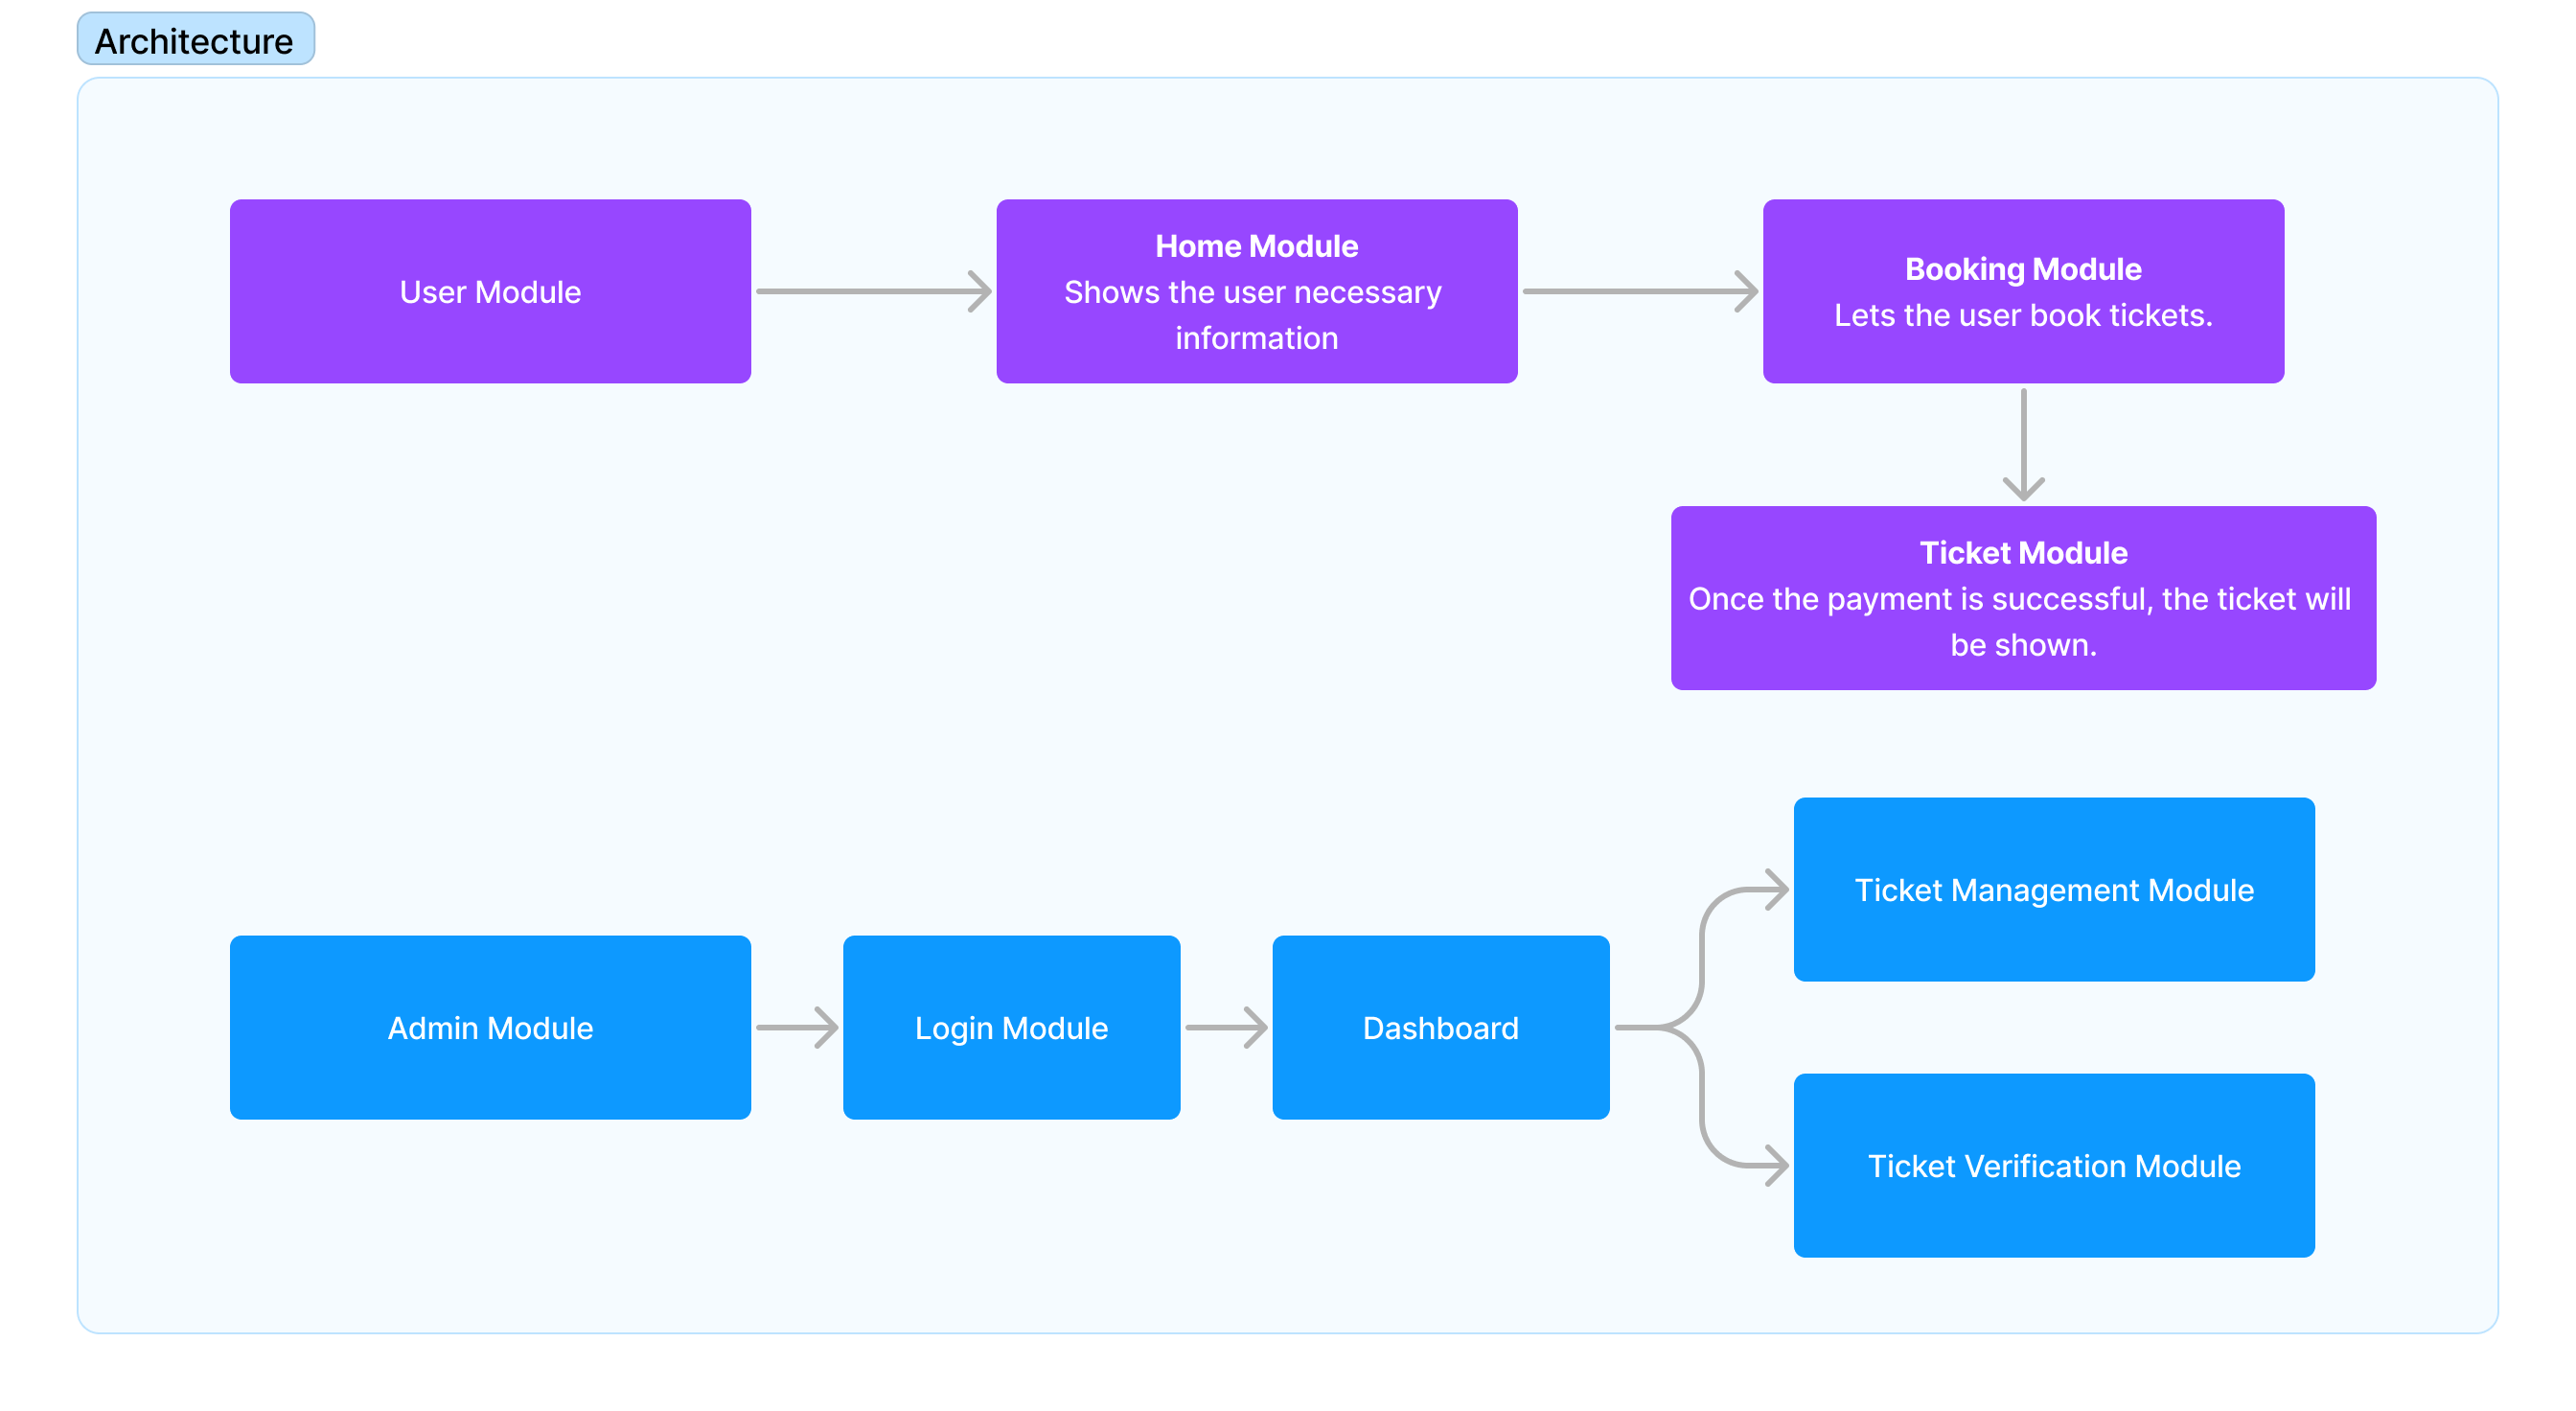
\includegraphics[width=\textwidth]{assets/Architecture.png}
    \caption{Architecture of the Proposed System}
    \label{architecture}
\end{figure}

\subsection{Data Flow Diagrams (DFD)}
The data flow diagram (DFD) maps out the flow of information for any process or system. It uses defined symbols like rectangles, circles, and arrows, plus short text labels, to show data inputs, outputs, storage points, and the routes between each destination. Data flowcharts can range from simple, even hand-drawn process overviews, to in-depth, multi-level DFDs that dig progressively deeper into how the data is handled.

Levels or layers are used in DFDs to represent progressive degrees of detail about the system or process. These levels include:
\begin{itemize}
    \item \textbf{Level 0}: Also known as a "context diagram," this is the highest level and represents a very simple, top-level view of the system being represented.
    \item \textbf{Level 1}: Still a relatively broad view of the system, but incorporates subprocesses and more detail.
    \item \textbf{Level 2}: Provides even more detail and continues to break down subprocesses as needed.
    \item \textbf{Level 3}: While this amount of detail is uncommon, complex systems can benefit from representation at this level.
\end{itemize}

In theory, more levels are possible, but they are rarely used and would likely represent more detail than a data flow diagram would normally convey. The diagrams of different levels of the DFD are illustrated in the following Figures
\begin{figure}[ht]
    \centering
    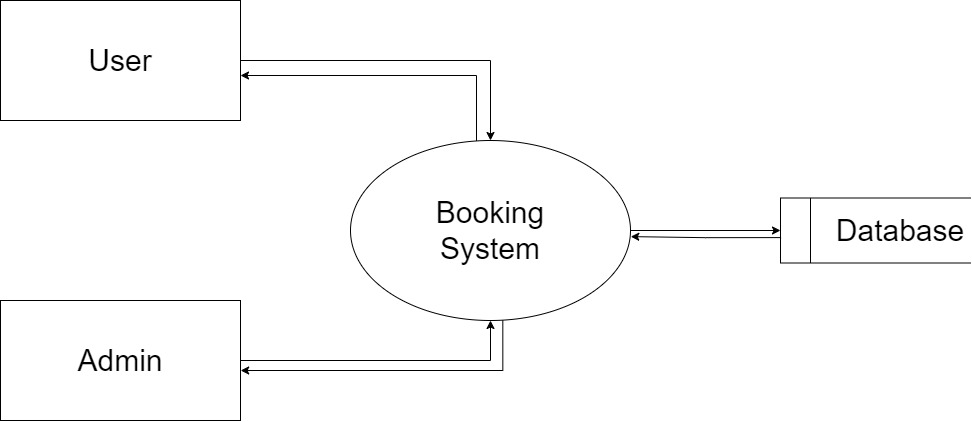
\includegraphics[width=\textwidth]{assets/DFD-1.jpg}
    \caption{Level 0 DFD}
    \label{dfd-1}
\end{figure}

\begin{figure}
    \centering
    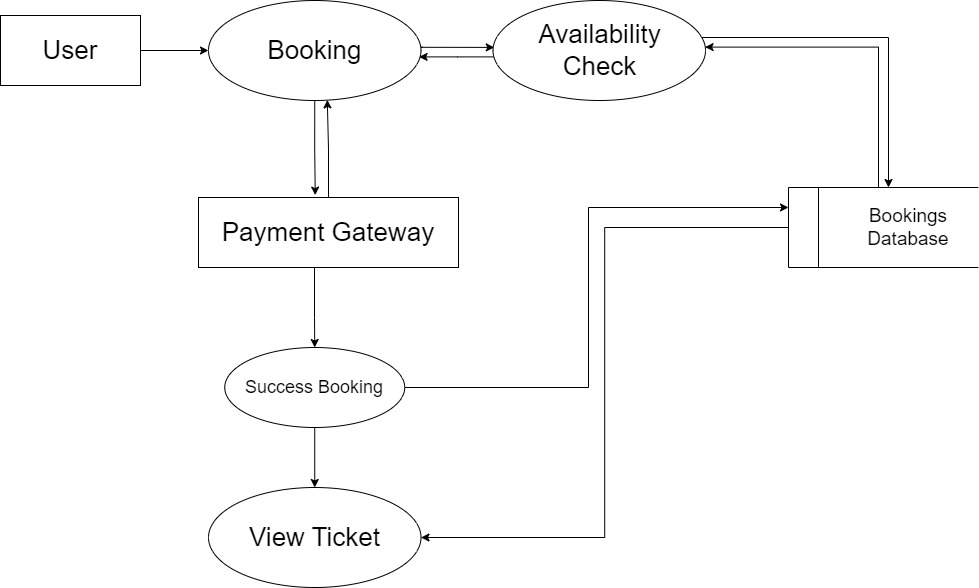
\includegraphics[width=\textwidth]{assets/DFD-2-User.jpg}
    \caption{Level 1 DFD - User Portal}
    \label{dfd-2-user}
\end{figure}

\begin{figure}
    \centering
    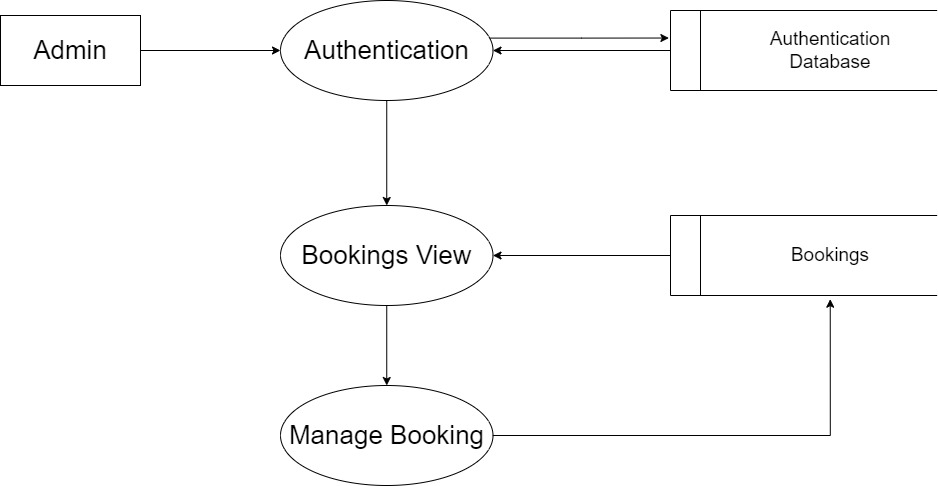
\includegraphics[width=\textwidth]{assets/DFD-2-Admin.jpg}
    \caption{Level 1 DFD - Admin App}
    \label{dfd-2-admin}
\end{figure}
\clearpage

\section{UML Diagrams}
UML stands for Unified Modeling Language. UML is a standardized general-purpose modeling language in the field of object-oriented software engineering. The standard is managed and was created by the Object Management Group. The goal is for UML to become a common language for creating models of object-oriented computer software. In its current form, UML is comprised of two major components: a Meta-model and a notation. In the future, some form of method or process may also be added to or associated with UML.
The Unified Modeling Language is a standard language for specifying, visualization, constructing, and documenting the artifacts of software systems, as well as for business modeling and other non-software systems. The UML represents a collection of best engineering practices that have proven successful in the modeling of large and complex systems. UML is a very important part of developing object-oriented software and the software development process. The UML uses mostly graphical notations to express the design of software projects.

The primary goals in the design of the UML are as follows:
\begin{itemize}
    \item Provide users with a ready-to-use, expressive visual modeling language so that they can develop and exchange meaningful models.
    \item Provide extensibility and specialization mechanisms to extend the core concepts.
    \item Be independent of particular programming languages and development processes.
    \item Provide a formal basis for understanding the modeling language.
    \item Encourage the growth of the object-oriented tools market.
    \item Support higher-level development concepts such as collaborations, frameworks, patterns, and components.
    \item Integrate best practices.
\end{itemize}

% -- Chapter 4 ----------------------------

\chapter{System Testing and Deployment}
In broad terms, system testing ensures the efficient and seamless performance of a system. It involves testing a program to uncover potential errors that could adversely impact its future functionality. Successful test cases are those that have a high likelihood of revealing errors, thereby aiding in the identification and resolution of previously unknown issues.

\section{Test Cases}
As previously discussed, testing is the methodical process of identifying potential vulnerabilities in the finalized software product. It involves evaluating the performance of sub-assemblies, components, assemblies, and the entire product to ensure alignment with business requirements and user expectations while minimizing the risk of sudden failure. Today, various types of tests are employed, each serving distinct testing objectives.

\section{Testing Techniques}
A test plan serves as a comprehensive document outlining the strategy, scope, resources, and schedule for planned testing activities. It delineates various test items, including the features to be tested, associated tasks, assignment of responsibilities, level of tester autonomy, testing environment specifications, design techniques, and exit criteria. Additionally, it addresses emergency risk mitigation strategies. Essentially, it records the test planning process and typically involves significant input from test engineers. The following sections describe different testing techniques in detail.

\begin{itemize}
    \item \textbf{Unit Testing:}
          Unit testing involves designing test cases to validate the internal logic of the program. This includes verifying all decision branches and internal code. Unit testing occurs after the completion of individual units and before integration. It focuses on conducting basic-level tests at the component stage, assessing specific business processes, and system configurations. The goal of unit testing is to ensure that each unique path of the process executes accurately according to documented specifications, with clearly defined inputs and expected results.
    \item \textbf{Integration Testing:}
          Integration testing focuses on evaluating integrated software components to ensure they function as a cohesive program or application. It employs an event-driven approach, primarily concerned with assessing the overall behavior of the system. Integration tests validate that the components, which have already passed successful unit testing, work together effectively. This type of testing is specifically designed to uncover any issues that may arise from the combination of components.
    \item \textbf{Functional Testing}:
          Functional testing ensures that the system's functions are systematically verified against technical requirements, system documentation, and user manuals. It aims to provide a comprehensive validation of the system's functionality, ensuring that all specified functions are available and operate according to established criteria.
    \item \textbf{System Testing}
          System testing, as its name implies, is a form of testing that verifies whether the software system aligns with the established business requirements and objectives. This testing phase includes the examination of system configurations to ensure consistent and predictable outcomes, along with the analysis of system behavior. System testing is reliant
    \item \textbf{White Box Testing}
          White box testing involves examining the internal components of the system software, allowing testers to access and manipulate them directly. This testing approach is inherently complex, requiring testers to analyze data structures, components, and other internal elements to identify potential bugs or errors. White box testing is employed when black box testing is insufficient in uncovering bugs. Due to its intricacy, white box testing typically requires more time to implement effectively.
    \item \textbf{Black Box Testing}
          Black box testing involves assessing the software system based solely on its inputs and outputs, without access to its internal components. This testing method is straightforward, as testers focus on the system's behavior rather than its internal structure. Even testers with basic programming knowledge can conduct black box testing effectively. Compared to white box testing, black box testing is less time-consuming and is particularly suitable for less complex and straightforward software. Additionally, it is generally less costly than white box testing.
    \item \textbf{Acceptance Testing}
          Acceptance testing, particularly user acceptance testing (UAT), is a pivotal stage in any project, requiring active involvement from end users. This testing phase is essential for ensuring that the system aligns with functional requirements and meets the expectations of its intended users.
\end{itemize}

\section{Criteria used for Testing of Proposed System}


\textbf{Entry Criteria:}
\begin{enumerate}
    \item \textbf{Completion of Website Development:} \\
          The development of the website using React is completed, ensuring all features and functionalities are implemented according to specifications.

    \item \textbf{Availability of Test Environment:} \\
          A test environment is set up with access to necessary tools and resources for conducting testing, including Jest for unit testing and Razorpay's test platform for payment system validation.

    \item \textbf{Team Readiness for Verification:} \\
          The project team is prepared to participate in verification sessions, including multiple team calls to review the system's functionality.
\end{enumerate}

\textbf{Testing Methodologies:}
\begin{enumerate}
    \item \textbf{White Box Testing (Unit Testing):} \\
          Utilizing Jest, the website undergoes white box testing to verify internal components and logic, ensuring adherence to coding standards and robustness.

    \item \textbf{Team Verification and Trial Runs:} \\
          Multiple team calls are scheduled to verify the system's functionality and address any issues identified during testing. Trial runs are conducted by DTPC authorities to assess the system's performance in real-world scenarios.

    \item \textbf{Payment System Testing with Razorpay:} \\
          Integration with Razorpay prompts thorough testing of the payment system, including transaction processing and error handling. Razorpay's test platform is utilized to validate the reliability and functionality of the payment gateway.
\end{enumerate}

\textbf{Exit Criteria:}
\begin{enumerate}
    \item \textbf{Successful Completion of Testing:} \\
          All identified test cases are executed, and the system demonstrates compliance with functional requirements and user expectations.

    \item \textbf{Resolution of Identified Issues:} \\
          Any issues or discrepancies uncovered during testing are addressed and resolved to ensure the system's stability and reliability.

    \item \textbf{Confirmation of Payment System Integration:} \\
          The payment system integration with Razorpay is successfully tested, and transactions are processed without errors or interruptions.
\end{enumerate}

Furthermore, in the development of the admin app, we employed a comprehensive testing approach to validate its functionality and robustness. This involved utilizing Flutter Unit Testing to scrutinize individual units of code, Widget Testing to assess the rendering and behavior of user interface components, and integration testing to evaluate the seamless interaction and integration of various modules within the app. By employing these testing methodologies, we ensured that the admin app meets the required standards of performance and functionality, contributing to a seamless user experience.

\section{Test Cases and Tools Used}

\begin{enumerate}
    \item \textbf{Unit Testing for Website (React):}
          \begin{itemize}
              \item \textbf{Tool:} Jest
              \item \textbf{Description:} Jest was utilized for unit testing the website components and internal logic, ensuring code robustness and adherence to coding standards.
          \end{itemize}

    \item \textbf{Integration Testing for Website (React):}
          \begin{itemize}
              \item \textbf{Description:} Integration testing was conducted to verify the seamless interaction and integration of different components within the website, ensuring overall system functionality.
          \end{itemize}

    \item \textbf{Payment System Testing (Razorpay):}
          \begin{itemize}
              \item \textbf{Tool:} Razorpay Test Platform
              \item \textbf{Description:} The payment system integration with Razorpay was rigorously tested using their test platform to validate transaction processing and error handling.
          \end{itemize}

    \item \textbf{Unit Testing for Admin App (Flutter):}
          \begin{itemize}
              \item \textbf{Tool:} Flutter's Built-in Testing Framework
              \item \textbf{Description:} Flutter's built-in testing framework was utilized for unit testing the admin app's individual units of code, ensuring code reliability and functionality.
          \end{itemize}

    \item \textbf{Widget Testing for Admin App (Flutter):}
          \begin{itemize}
              \item \textbf{Description:} Widget testing was performed to evaluate the rendering and behavior of UI components within the admin app, ensuring correct functionality and appearance.
          \end{itemize}

    \item \textbf{Integration Testing for Admin App (Flutter):}
          \begin{itemize}
              \item \textbf{Description:} Integration testing was conducted to verify the seamless interaction and integration of various modules within the admin app, ensuring overall system functionality.
          \end{itemize}
\end{enumerate}

By leveraging these testing tools and methodologies, thorough testing was conducted to validate the functionality, reliability, and performance of both the website and the admin app, ensuring a seamless user experience.

\chapter{CONCLUSIONS AND FUTURE WORK}

Reputation assessment stands as a critical element within online rating systems, garnering significant attention in numerous studies and research endeavors. Exploring various reputation measurement techniques has been pivotal in addressing the challenge of false reputation. While many existing works focus on evaluating product reputation through clustering, classification techniques, and hypothesis testing methods, few delve into assessing the confidence of ratings using suitable algorithms. Moreover, the complexity of evaluating both product and seller reputation adds another layer of challenge. In light of these considerations, the stature estimation framework not only assesses product reputation but also incorporates seller reputation evaluation. By determining the confidence of ratings and each seller's activity score, the framework enhances trustworthiness, allowing users to independently evaluate both products and sellers. Experimental results corroborate the efficacy of the stature estimation method in mitigating the impact of false reputation compared to conventional approaches like the arithmetic mean method.

Moving forward, there are several avenues for future work and system expansion. One potential direction is to extend the system to encompass the entirety of the Edakkal Caves website. This expansion could facilitate various enhancements, such as enabling the District Tourism Promotion Council (DTPC) Wayanad to disseminate event plans, additional information, and notifications to users. Additionally, further improvements to the website could include:
\begin{enumerate}
    \item Enhancing user experience through intuitive navigation and interactive features.
    \item Implementing personalized recommendation systems based on user preferences and past activities.
    \item Integrating social sharing functionalities to foster community engagement and user interaction.
    \item Incorporating multilingual support to cater to a diverse user base, thereby enhancing accessibility and inclusivity.
\end{enumerate}

By embarking on these future endeavors, the Ticket Booking System for Edakkal Caves can evolve into a comprehensive platform that not only facilitates efficient ticket booking but also serves as a valuable resource for tourists seeking information and experiences related to the Edakkal Caves and its surroundings.

\newpage
\pagenumbering{roman}
\setcounter{page}{6}
\nocite{*}
\bibliography{references}

\chapter*{APPENDICES}
\addcontentsline{toc}{chapter}{APPENDICES}
\pagenumbering{roman}
\setcounter{page}{7}
\renewcommand{\thesection}{\Alph{section}}

This section contains screenshots of various pages from the Ticket Booking System for Edakkal Caves application, providing visual representations of its user interface and functionality.


\begin{figure}[htbp]
    \centering
    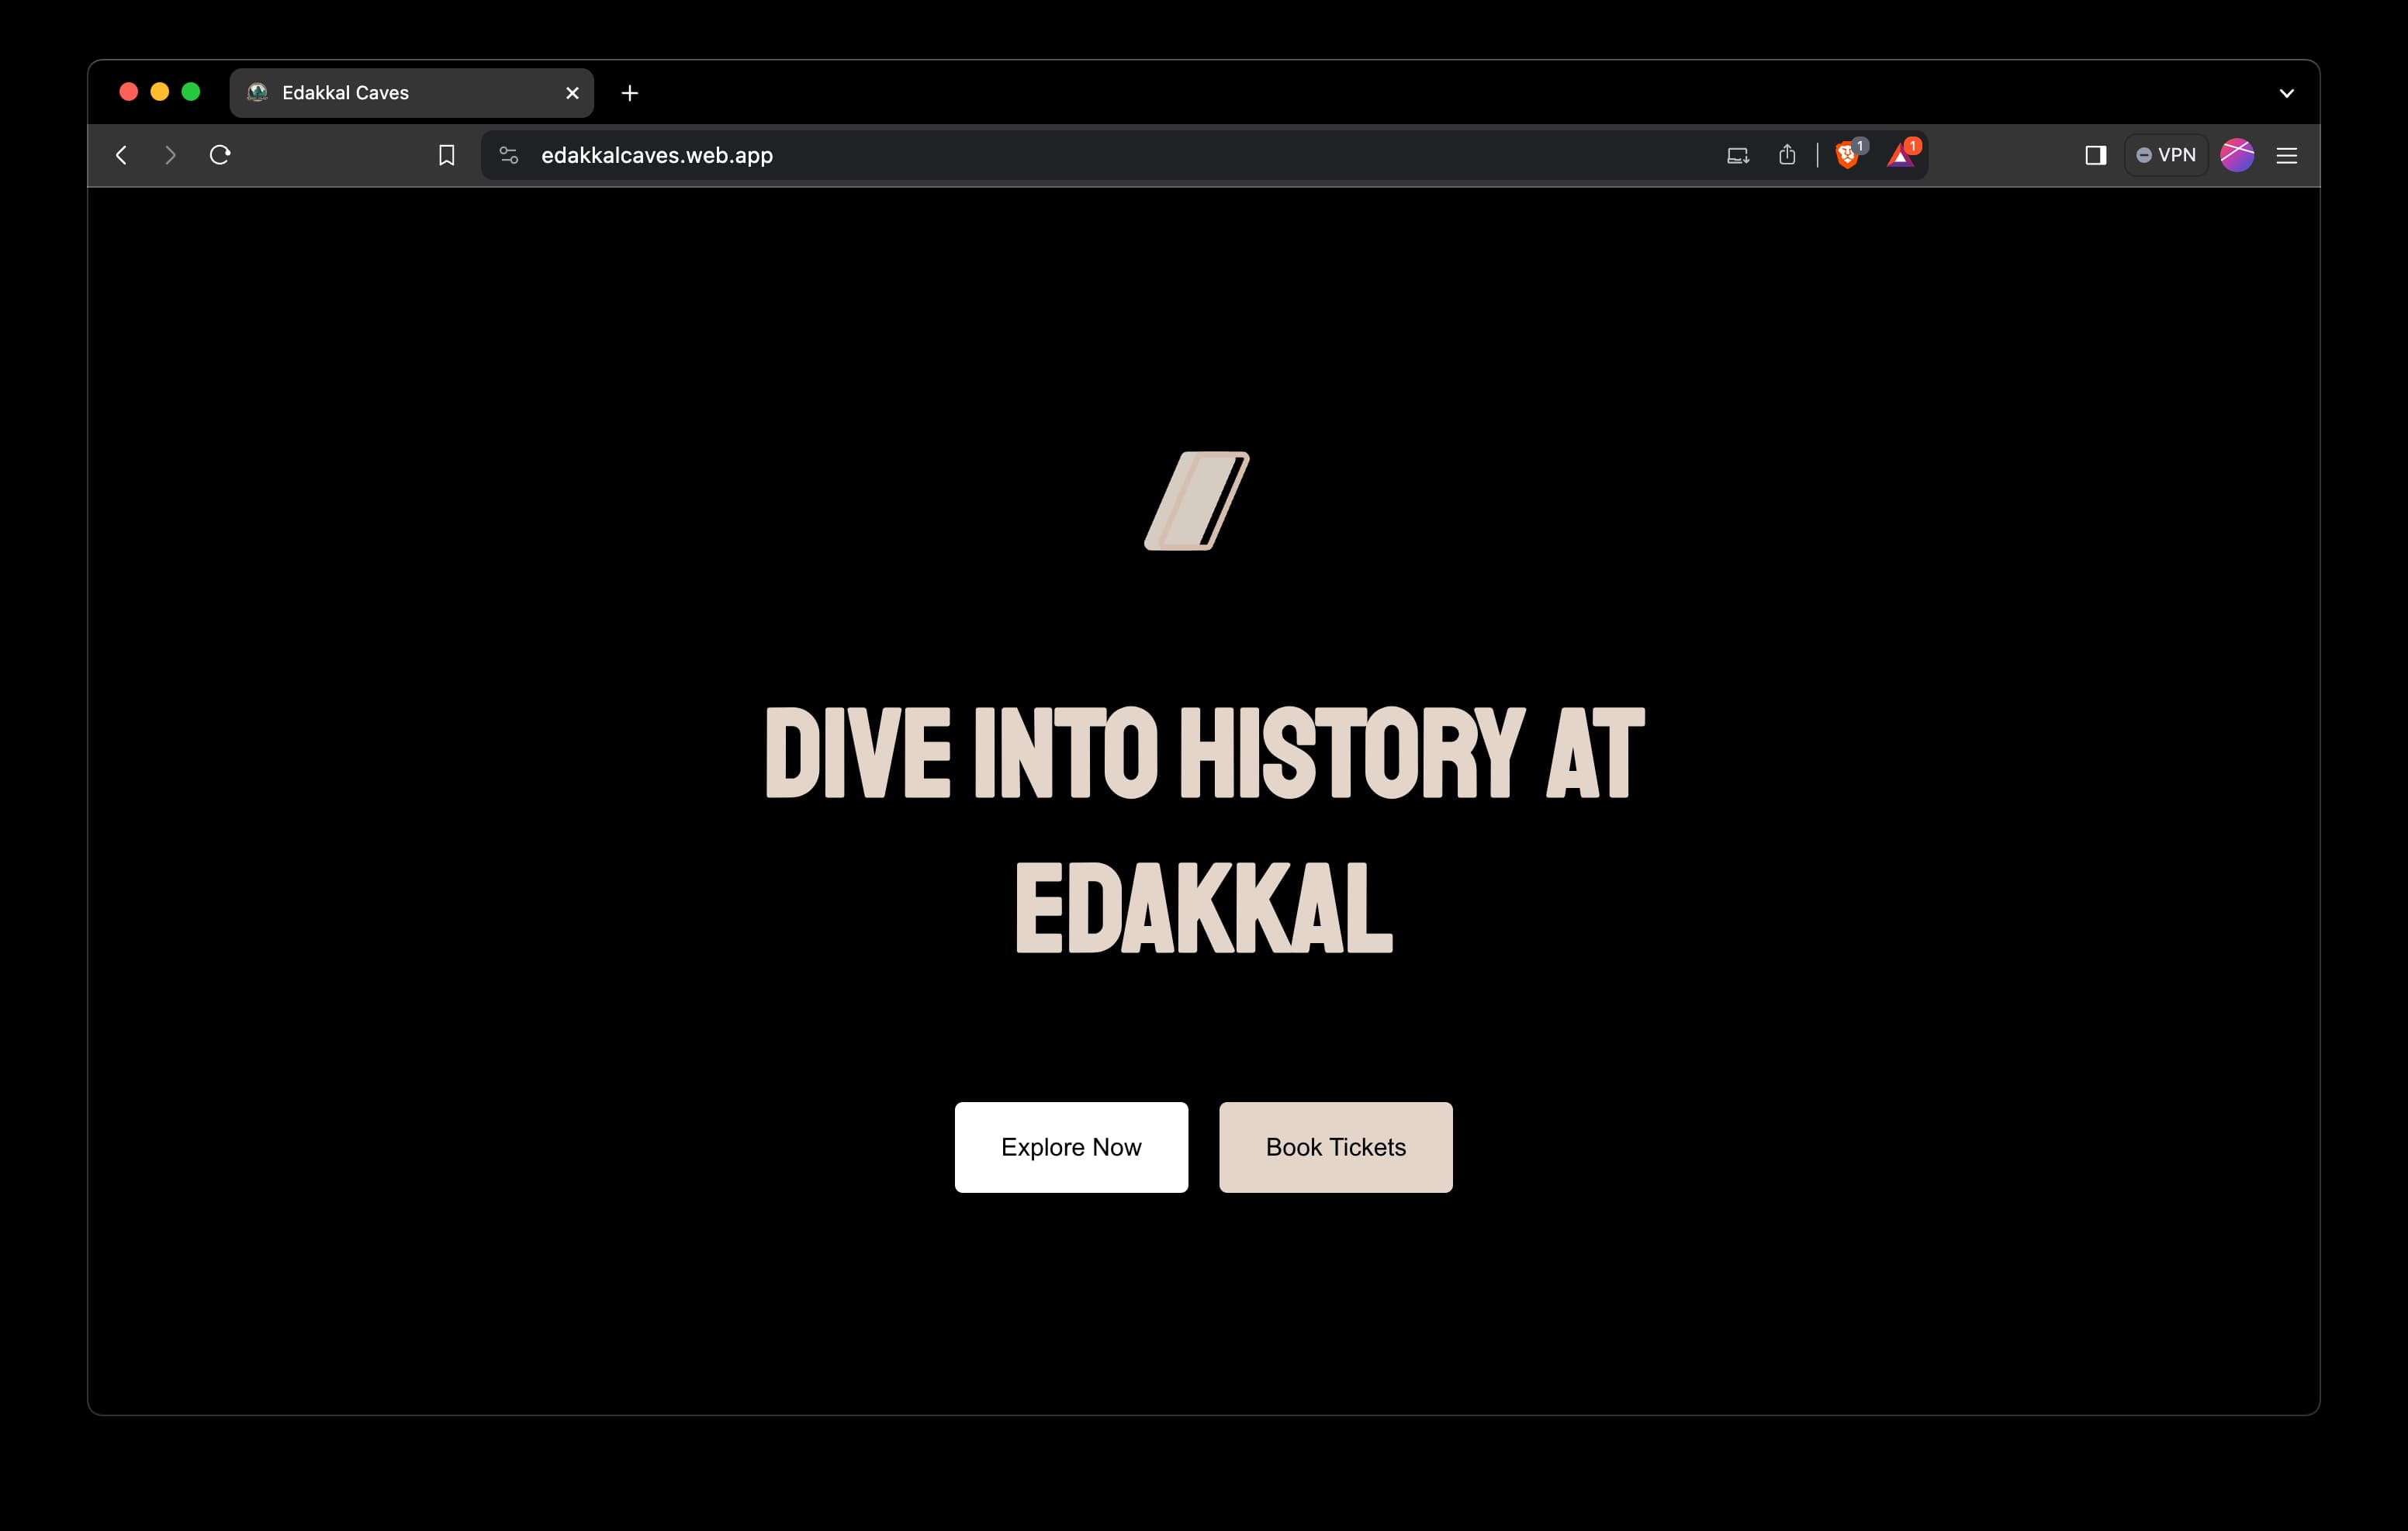
\includegraphics[width=1\textwidth]{screenshots/Home.jpg}
    \caption{Screenshot of the Home Page}
\end{figure}

\begin{figure}[htbp]
    \centering
    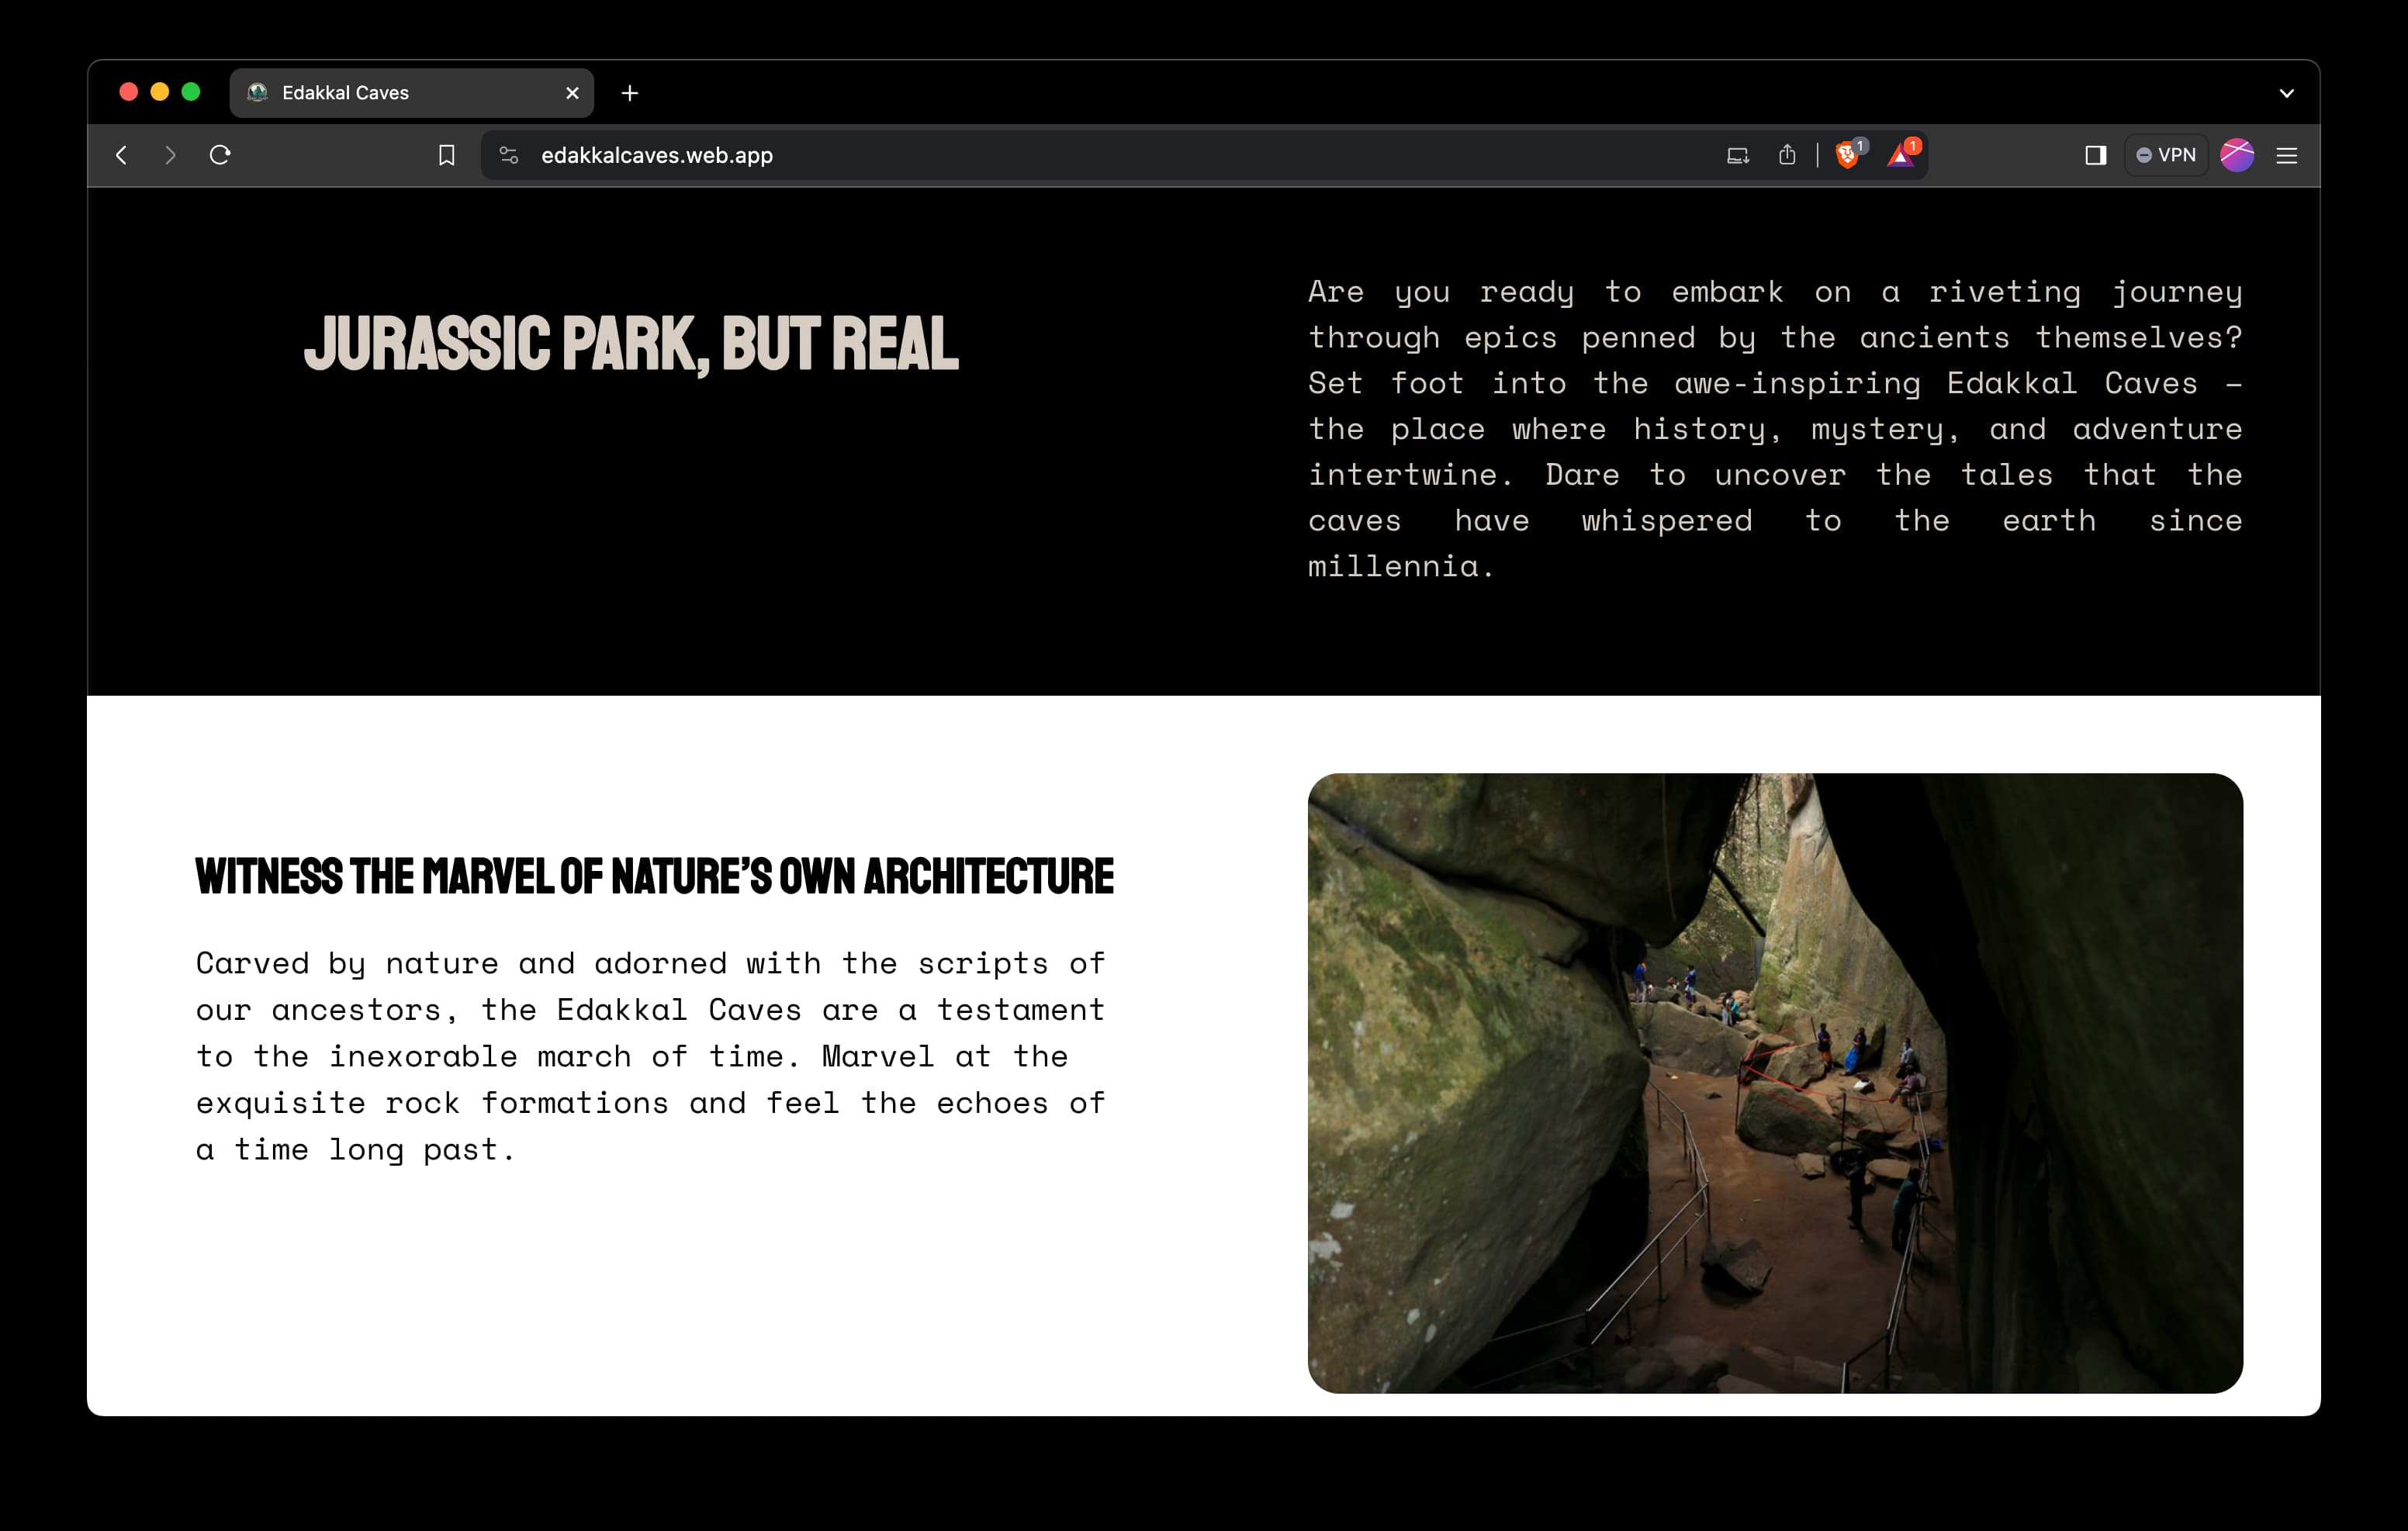
\includegraphics[width=1\textwidth]{screenshots/Home-2.jpg}
    \caption{Another Screenshot of the Home Page}
\end{figure}

\begin{figure}[htbp]
    \centering
    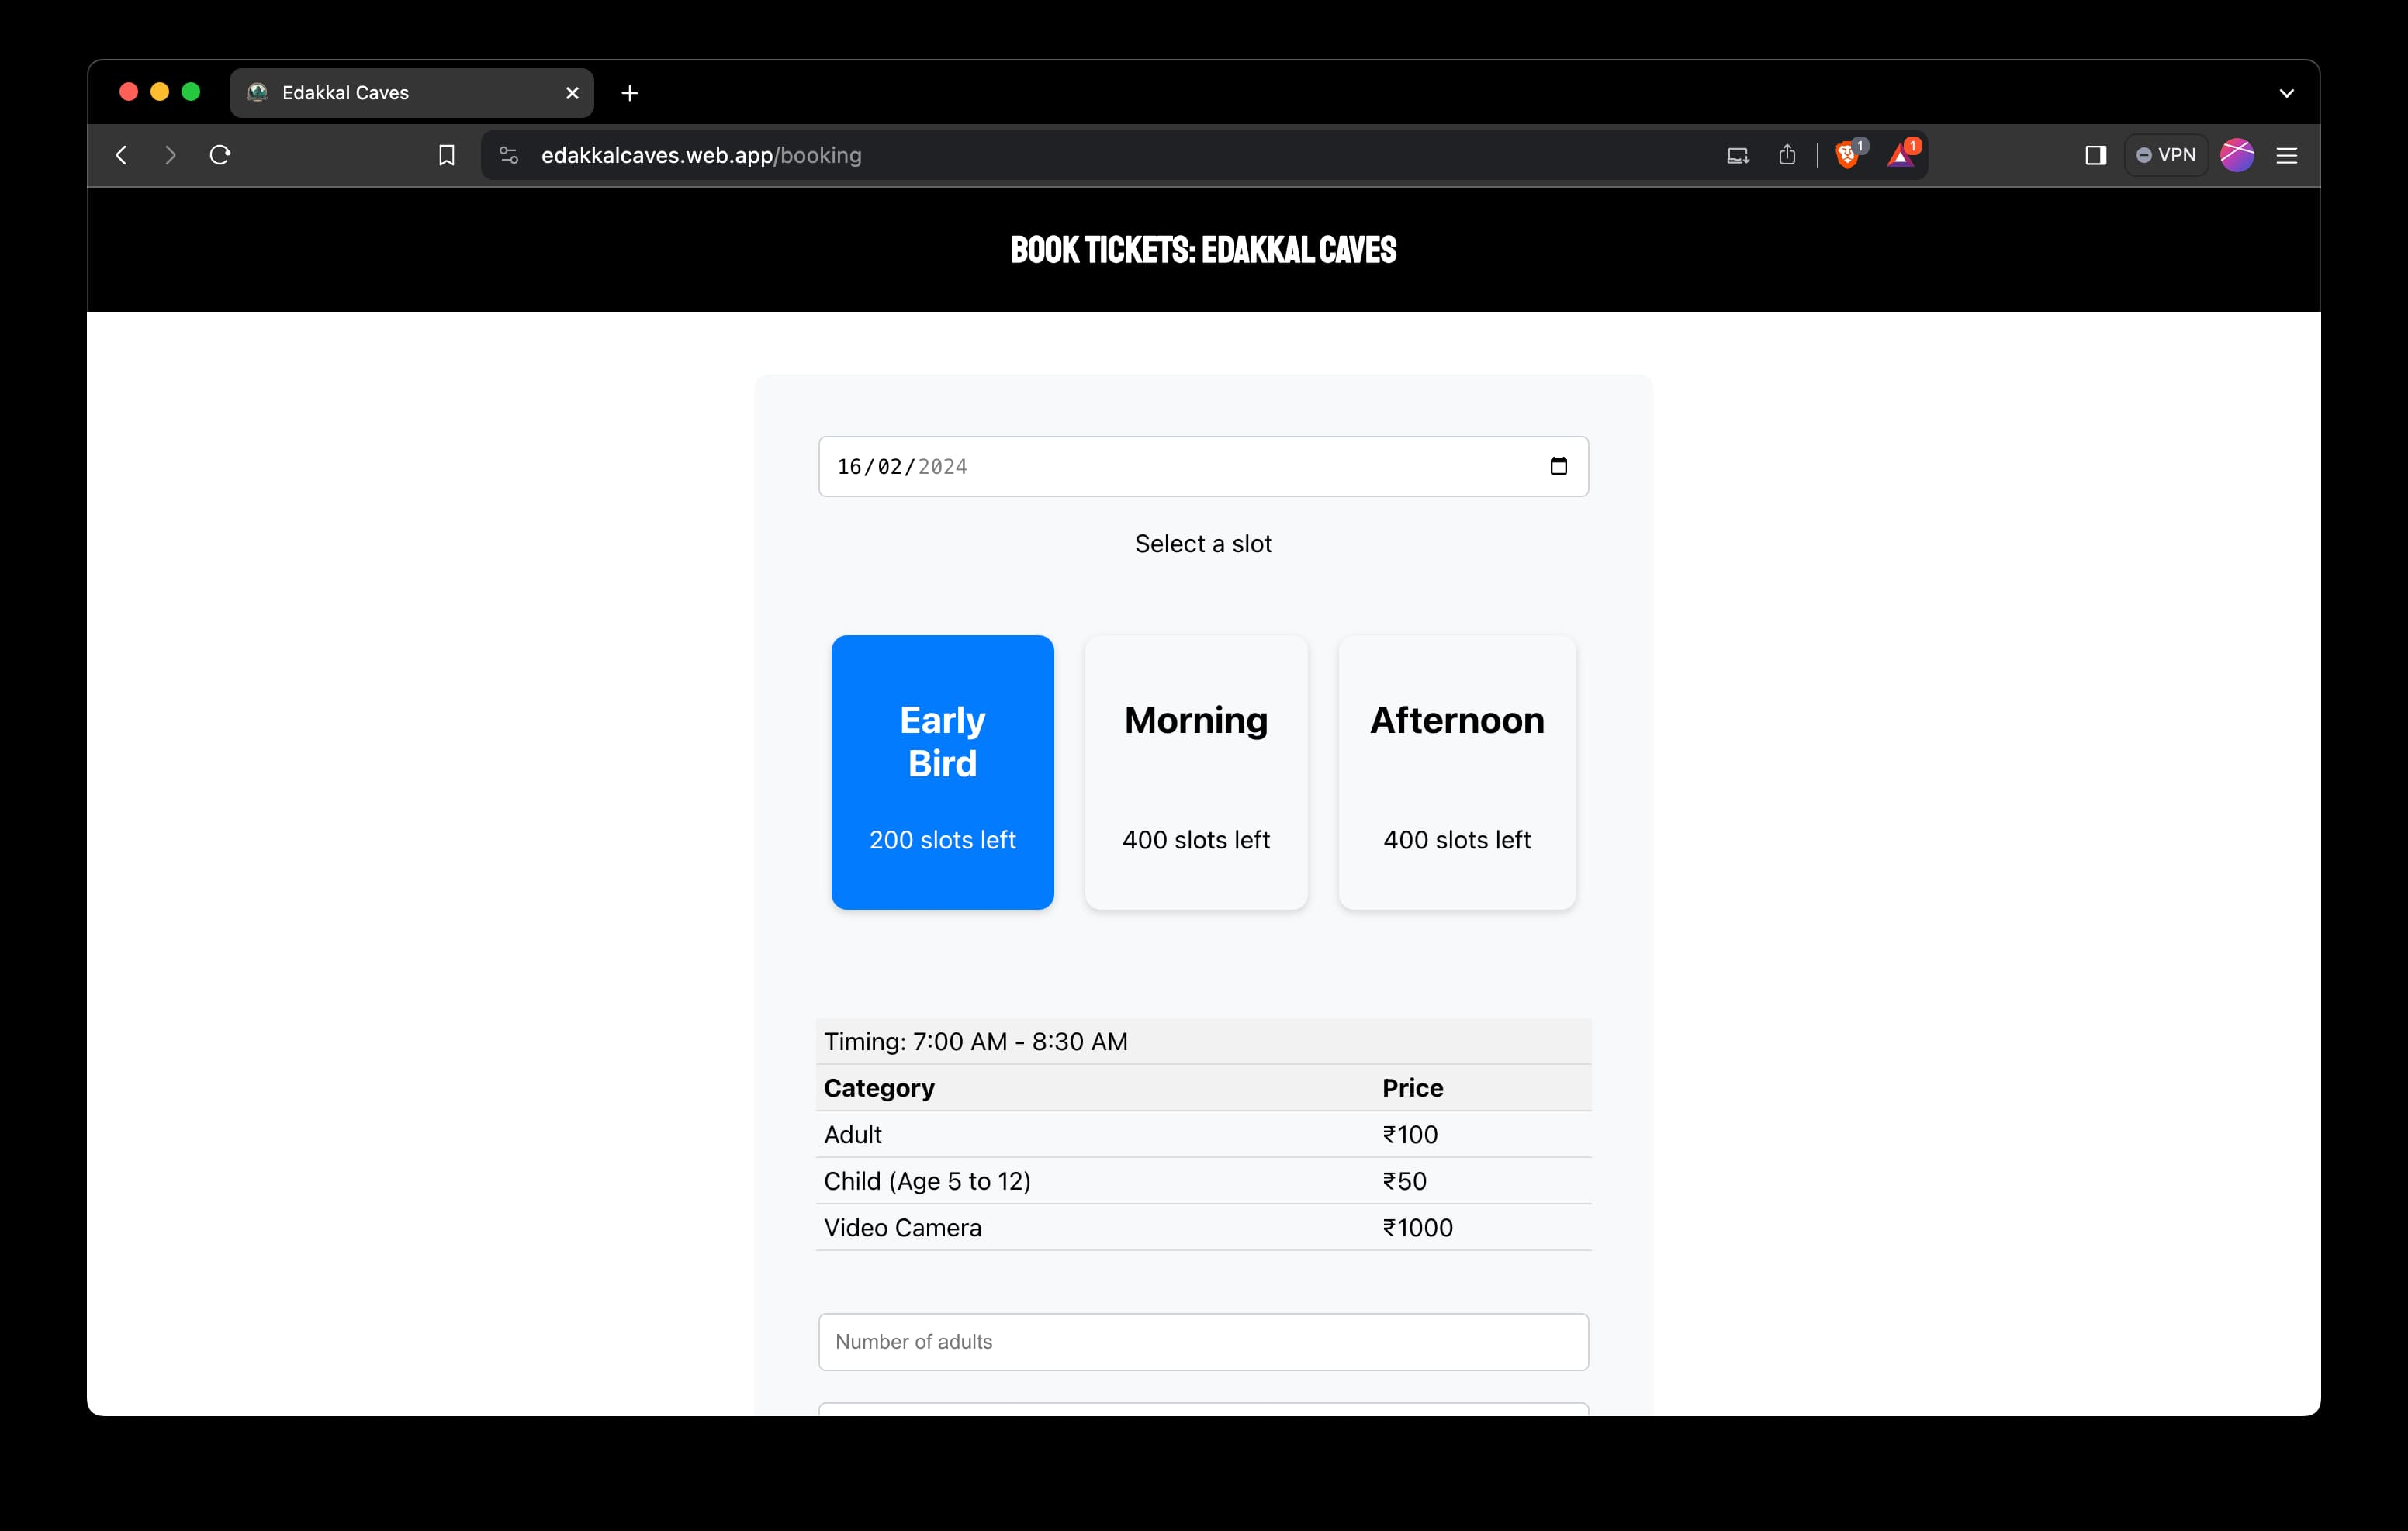
\includegraphics[width=1\textwidth]{screenshots/Booking.jpg}
    \caption{Screenshot of the Booking Page}
\end{figure}

\begin{figure}[htbp]
    \centering
    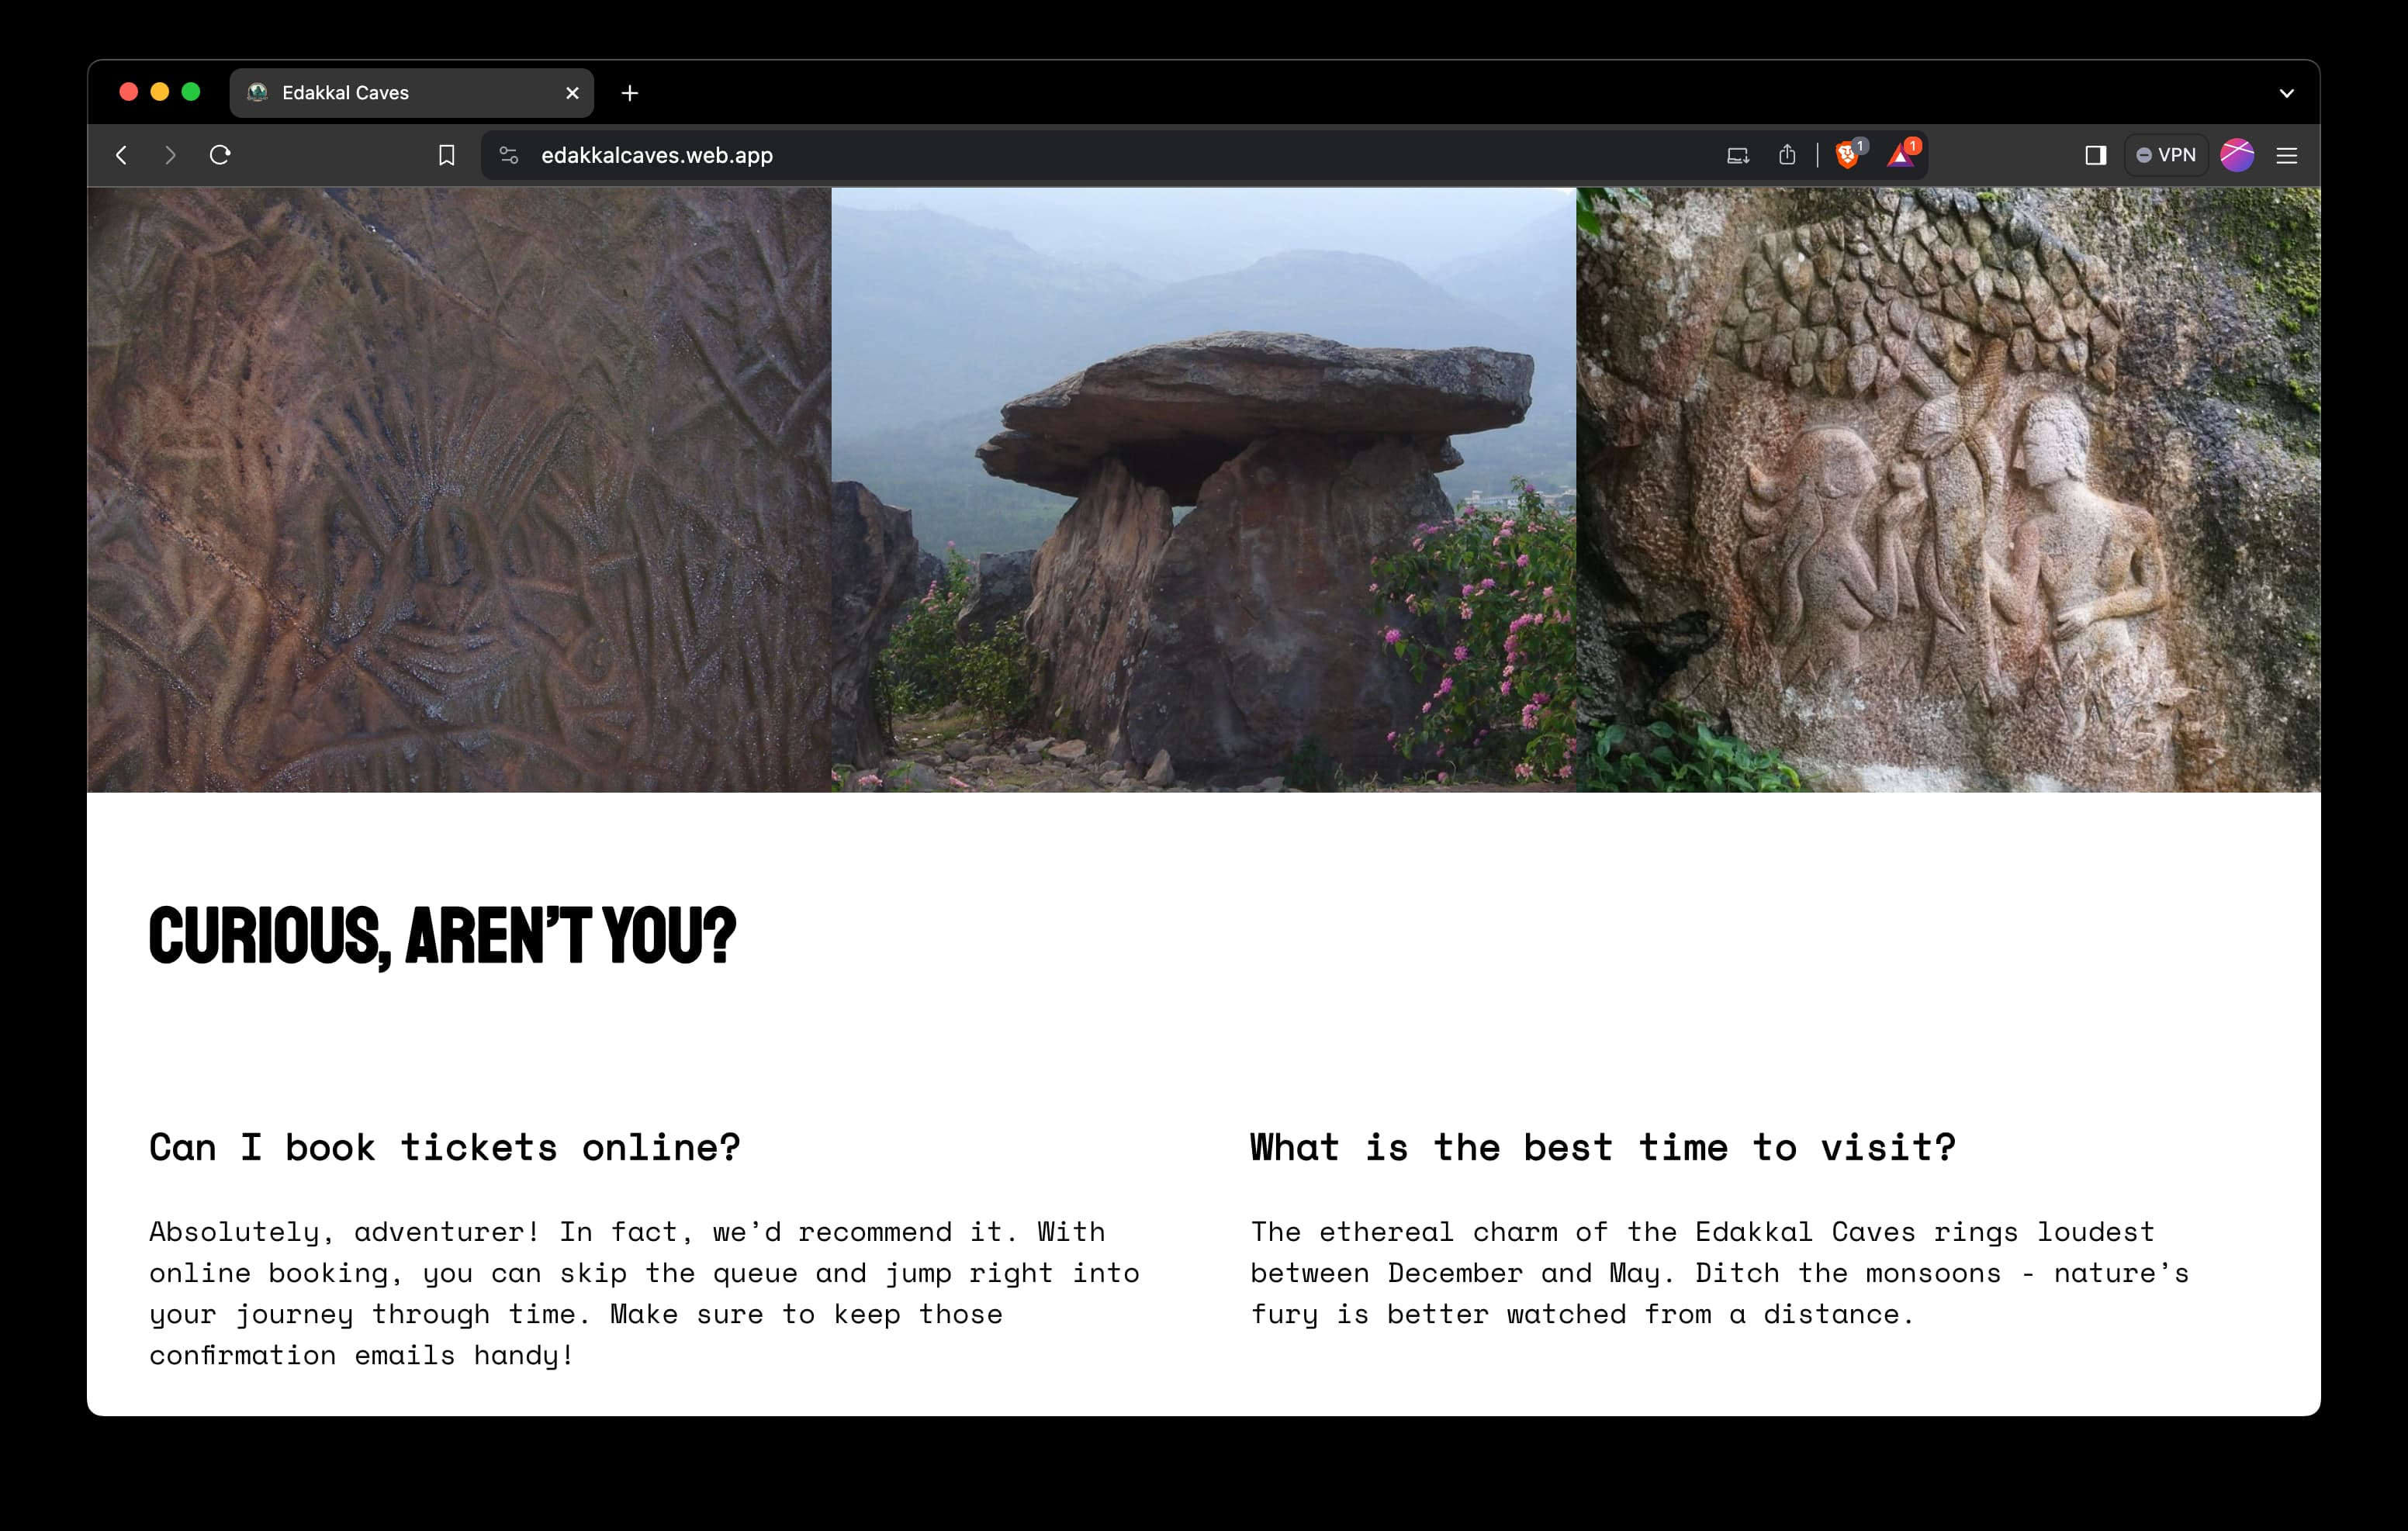
\includegraphics[width=1\textwidth]{screenshots/Gallery.jpg}
    \caption{Screenshot of the Gallery and FAQ section}
\end{figure}

\begin{figure}[htbp]
    \centering
    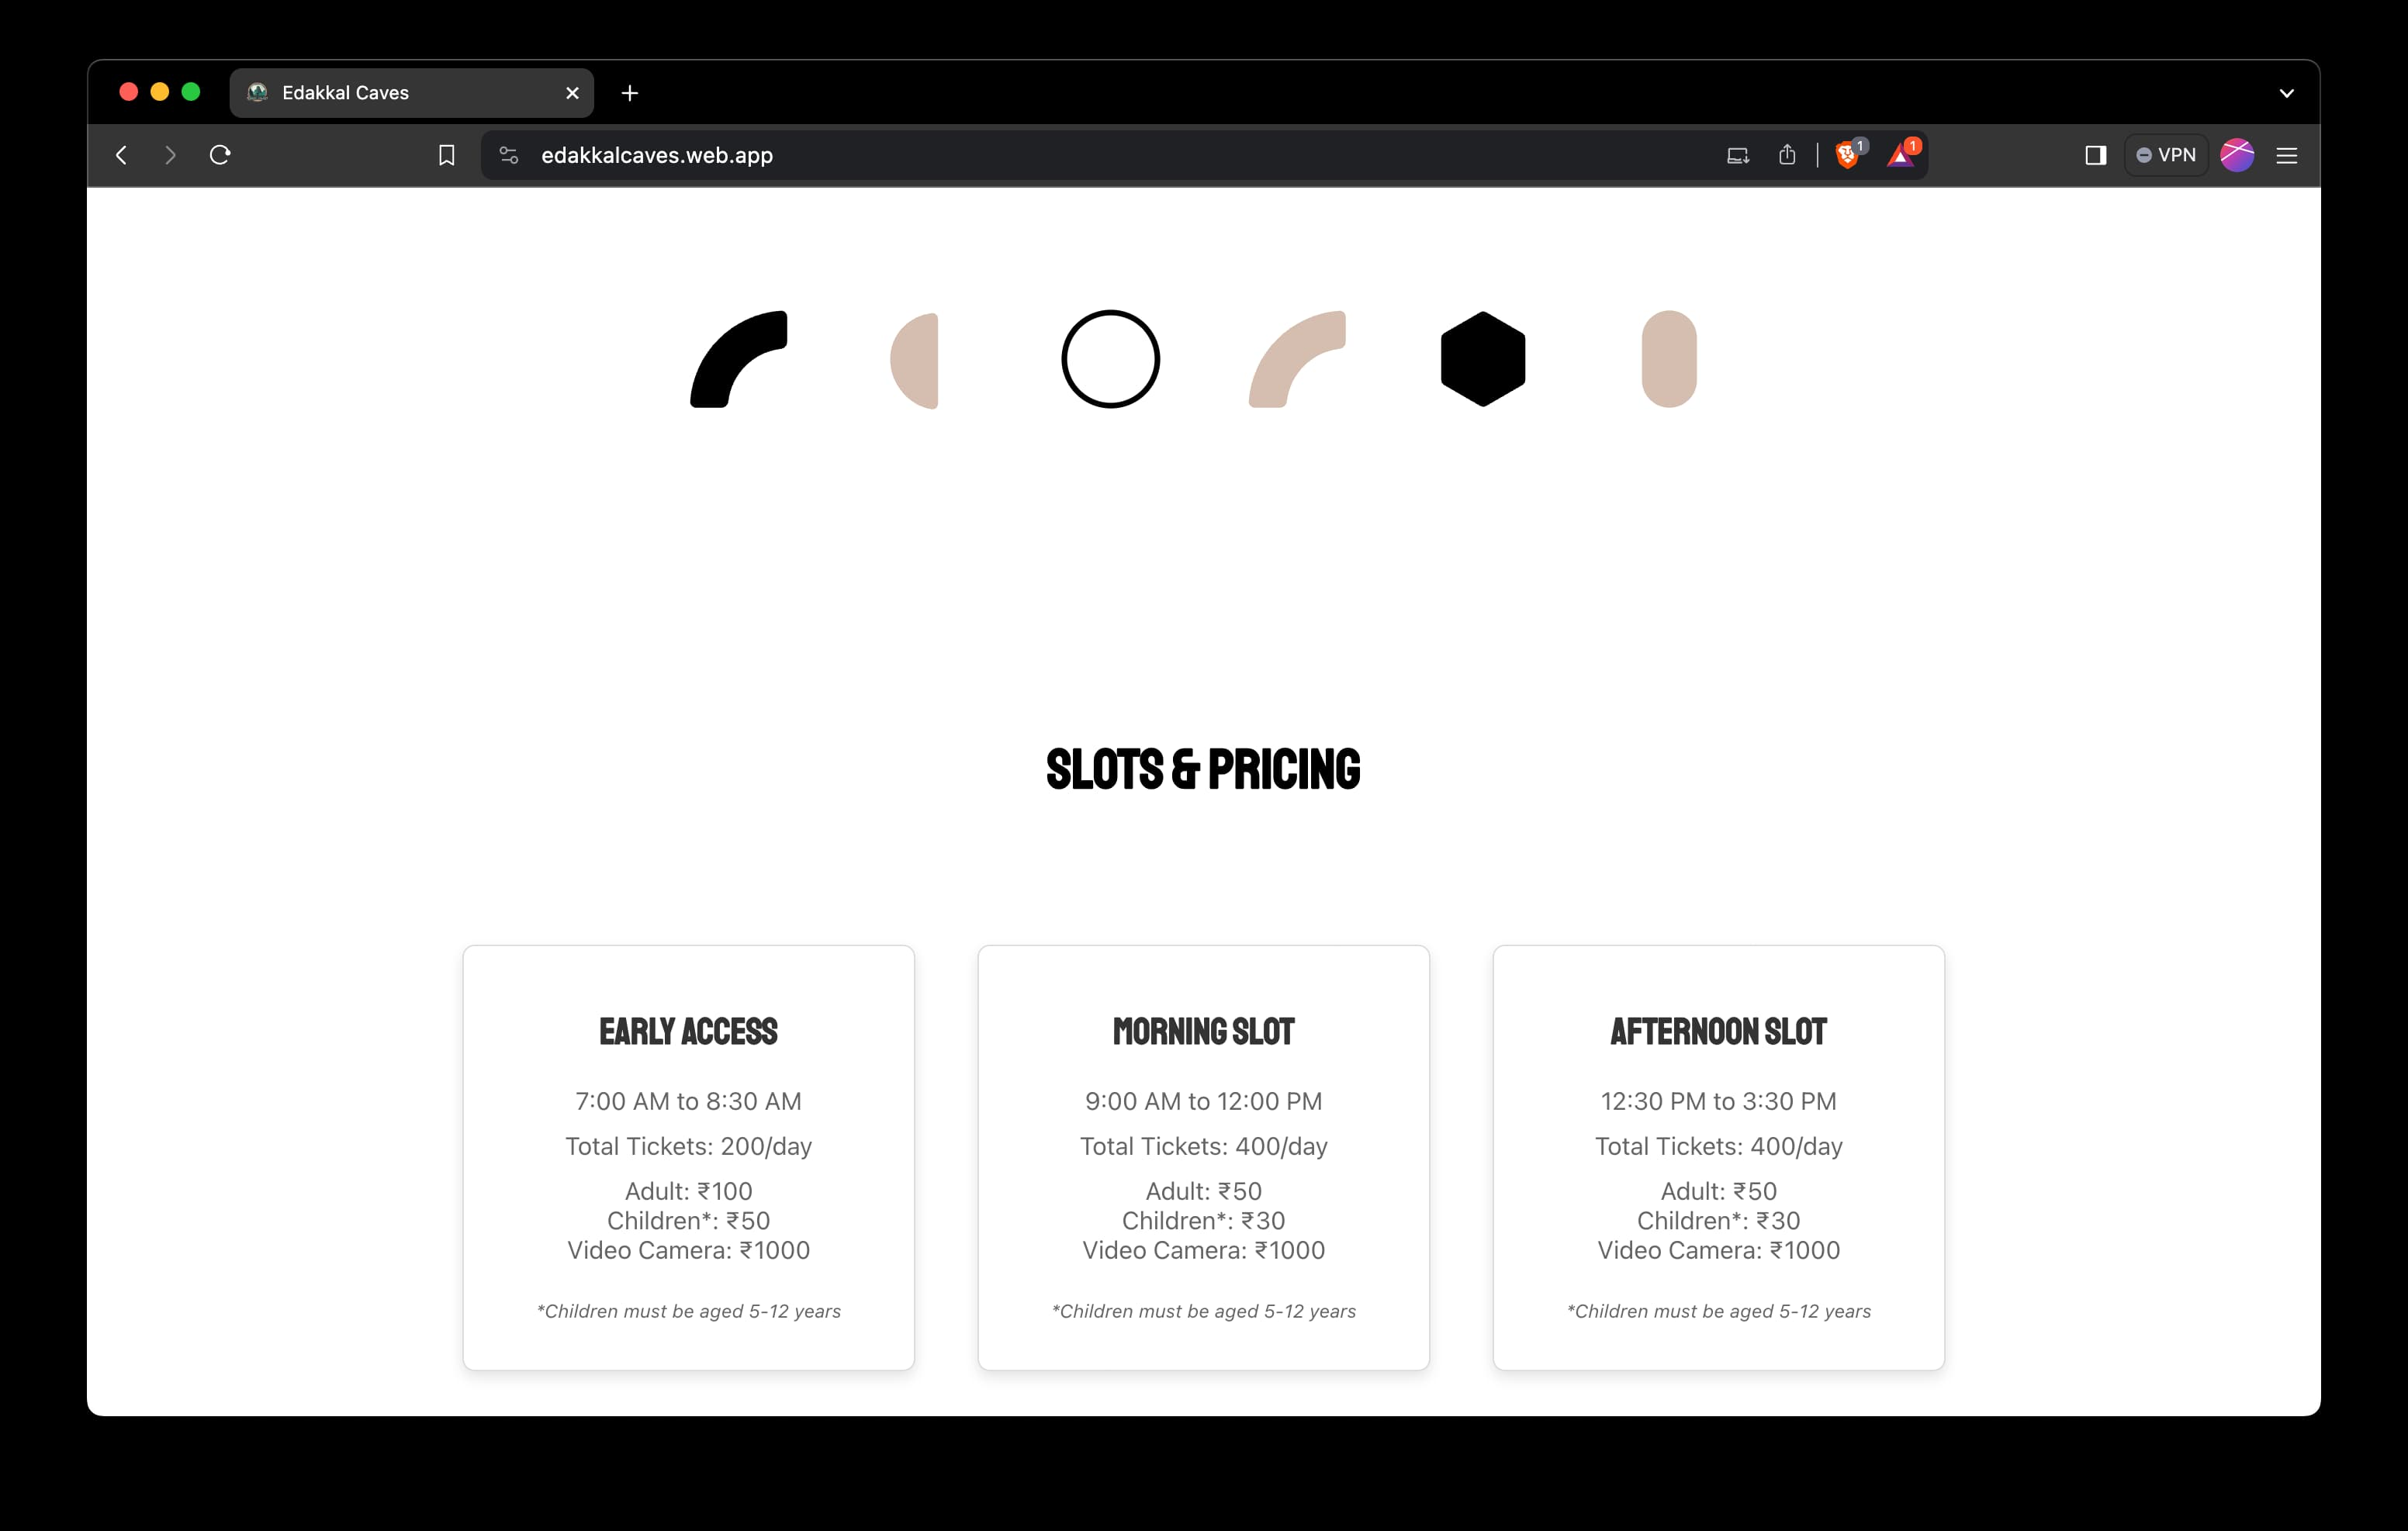
\includegraphics[width=1\textwidth]{screenshots/Slots.jpg}
    \caption{Screenshot of the section showing available slots}
\end{figure}

\begin{figure}[htbp]
    \centering
    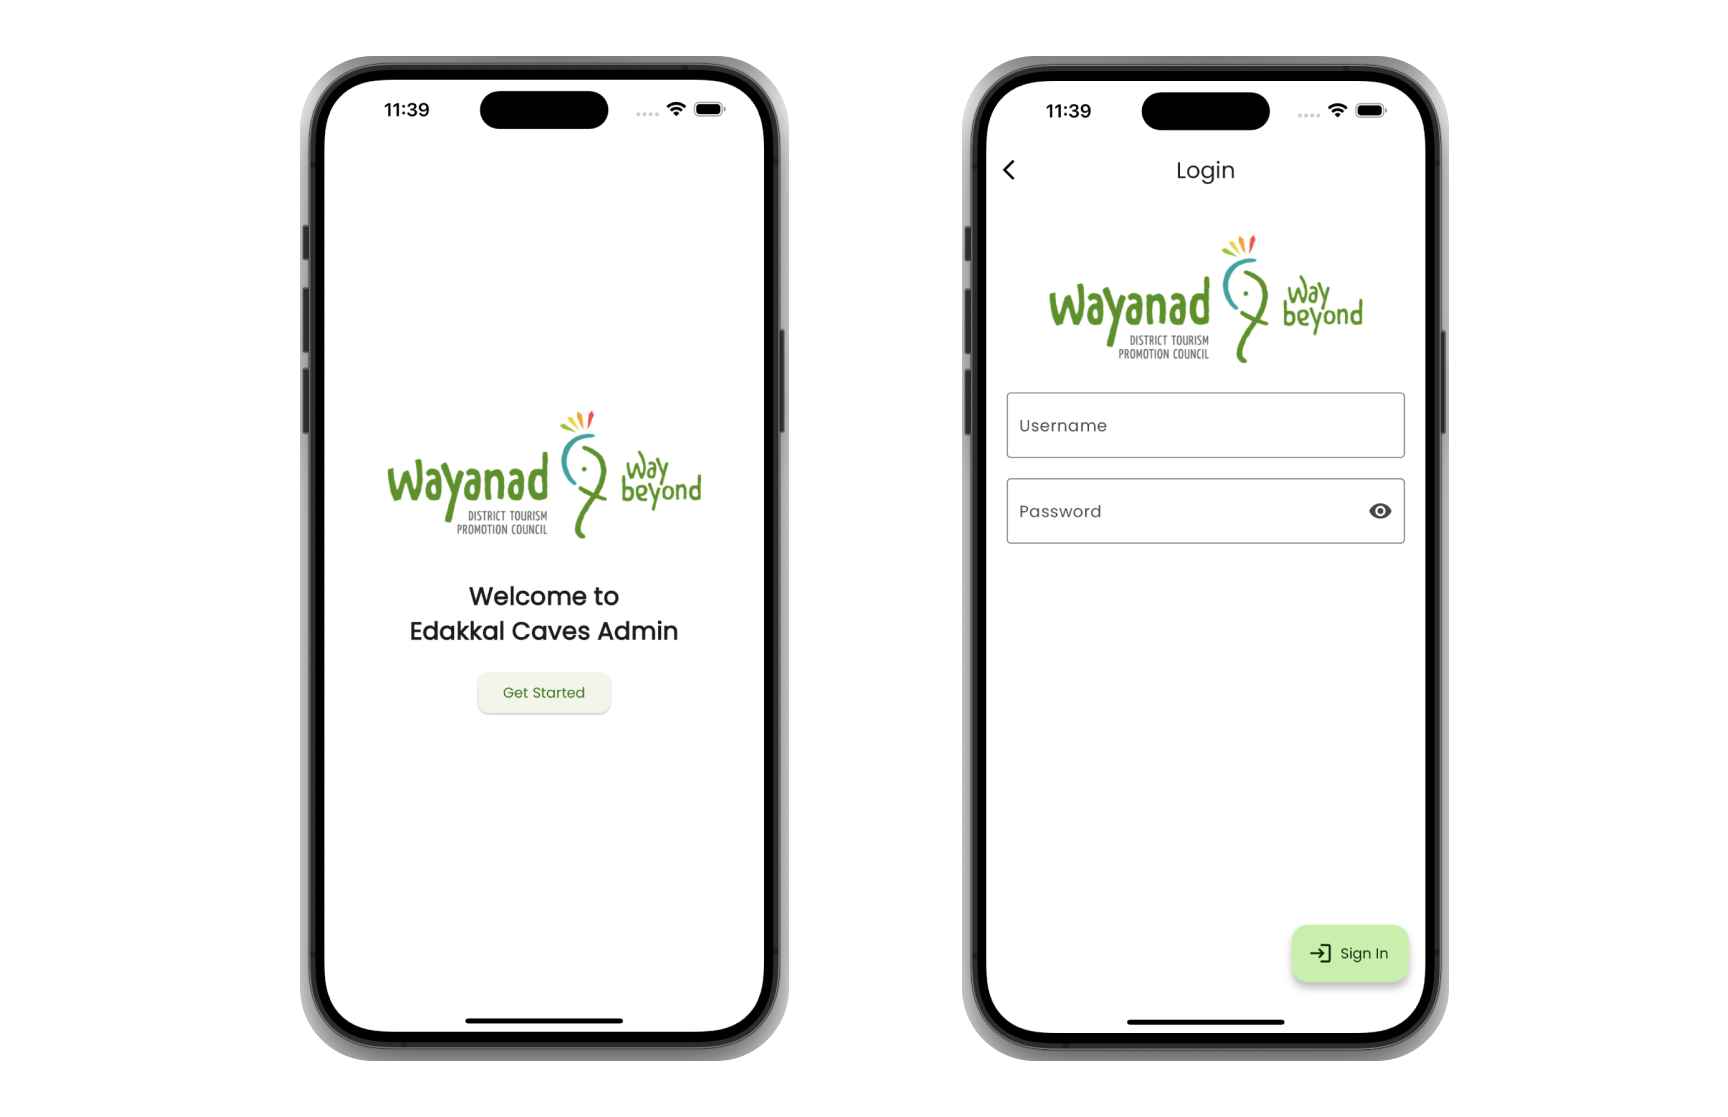
\includegraphics[width=1\textwidth]{screenshots/welcome-screens.png}
    \caption{Screenshot of the Welcome Screens}
\end{figure}

\begin{figure}[htbp]
    \centering
    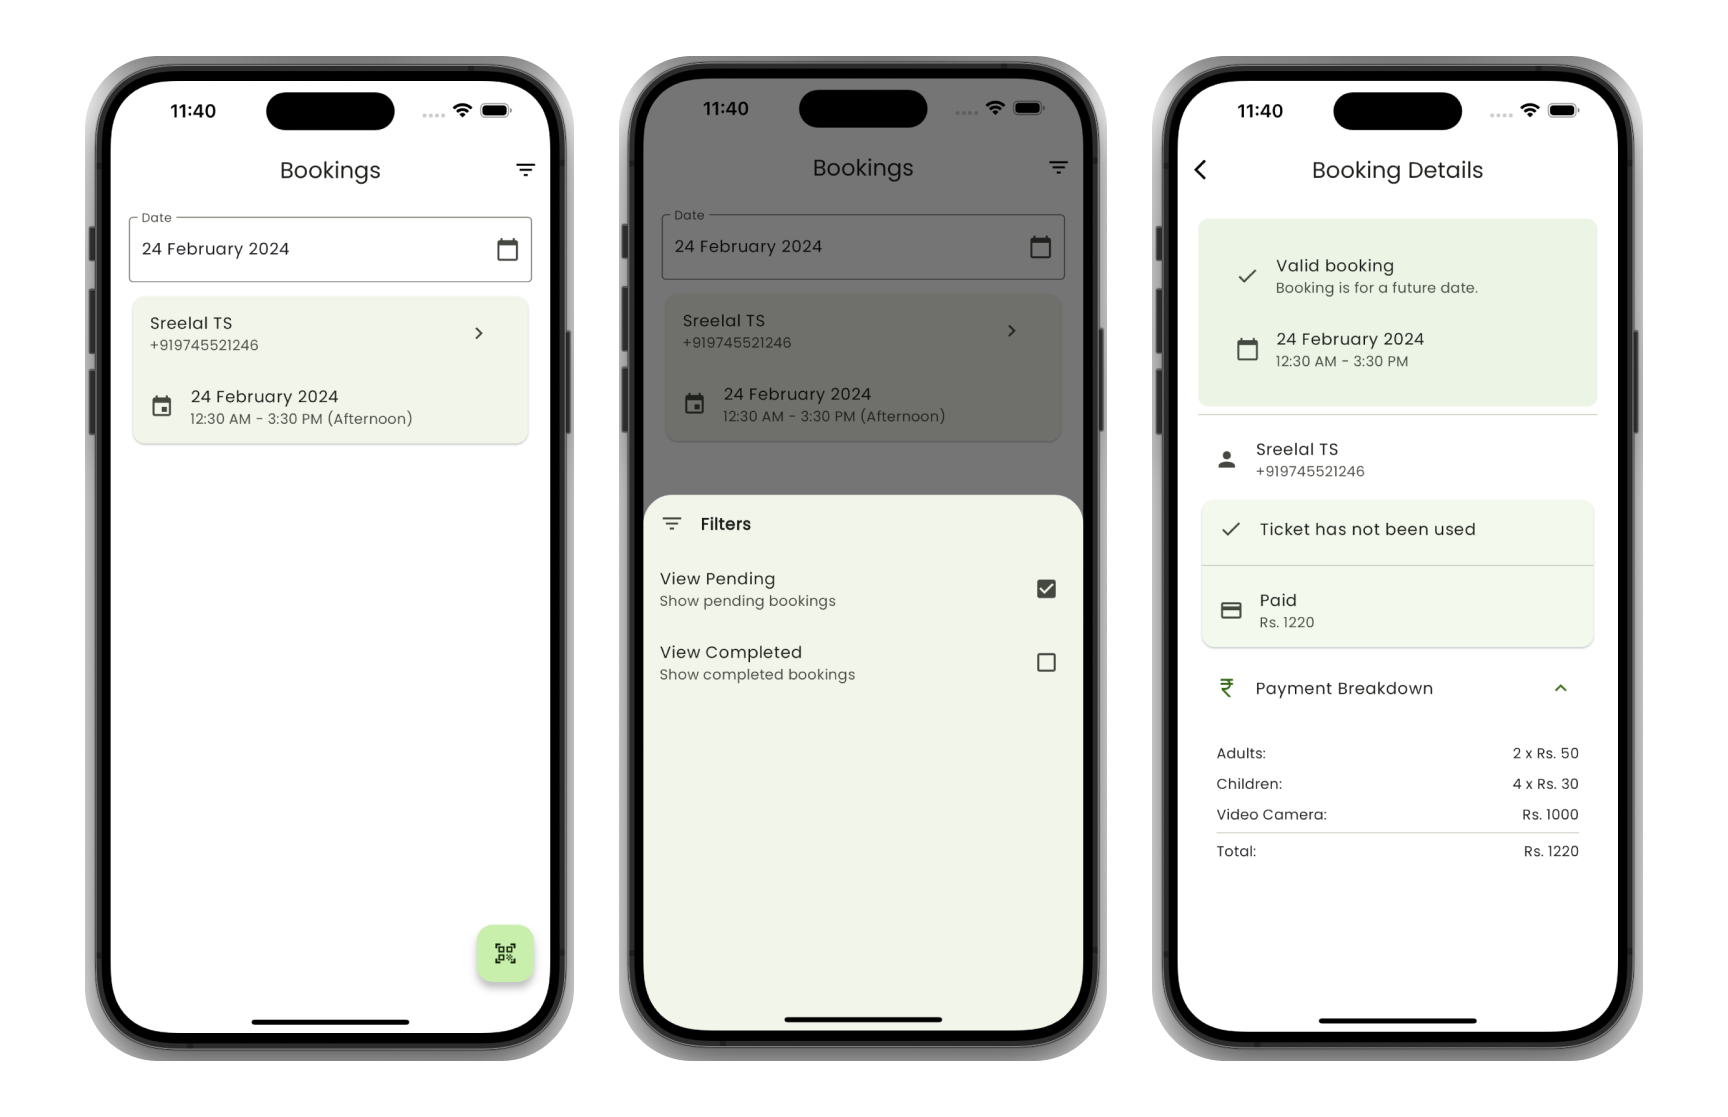
\includegraphics[width=1\textwidth]{screenshots/admin-app-screens.png}
    \caption{Screenshot of the Admin App Screen}
\end{figure}

\end{document}
